\documentclass[12pt]{report}
% English hyphenation
\usepackage[british]{babel}
% Links
\usepackage[breaklinks=true]{hyperref}
% Images
\usepackage{graphicx}
\graphicspath{ {./images/} }

\usepackage[noabbrev]{cleveref}

\crefname{appsec}{Appendix}{Appendices}

\usepackage[utf8]{inputenc}
\usepackage{csquotes}

\usepackage{esdiff}

\usepackage{caption}
\usepackage{subcaption}
\usepackage[a4paper, headheight=15pt]{geometry}

\usepackage[load-configurations=abbreviations, binary-units=true]{siunitx}

\usepackage{fancyhdr}
\pagestyle{fancy}
\fancyhead{}
\fancyhead[L]{\leftmark}
\fancyhead[R]{\rightmark}
\fancyfoot{}
\fancyfoot[C]{\thepage}
\renewcommand{\headrulewidth}{0.4pt}
\renewcommand{\footrulewidth}{0.4pt}
\renewcommand{\chaptermark}[1]{ \markboth{#1}{} }
\renewcommand{\sectionmark}[1]{ \markright{#1}{} }

% Source images
\newcommand{\imagesource}[1] {\caption*{\begin{footnotesize} Source: \url{#1} \end{footnotesize}}}

% Appendix
\usepackage[toc,page]{appendix}
% Change name of toc
\renewcommand*\contentsname{Table of Contents}

\usepackage[style=numeric,sorting=none]{biblatex}
\addbibresource{bibliography.bib}

\title{Shape Tracking Spiking Neural Network}
\author{Filippo Ferrari}
\date{April 2019}


\begin{document}

\begin{titlepage}
	\newcommand{\HRule}{\rule{\linewidth}{0.5mm}} % Defines a new command for horizontal lines, change thickness here
	
	\center % Centre everything on the page
	
	%------------------------------------------------
	%	Headings
	%------------------------------------------------
	
	\textsc{\LARGE University of Manchester}\\[1cm] % Main heading such as the name of your university/college
	
	\textsc{\Large School of Computer Science}\\[1.5cm] % Major heading such as course name
	
	
	%------------------------------------------------
	%	Title
	%------------------------------------------------
	
	\HRule\\[0.4cm]
	
	{\huge\bfseries Shape Tracking\\
	Spiking Neural Network}\\[0.4cm] % Title of your document
	
	\HRule\\[2.0cm]
	
	%------------------------------------------------
	%	Author(s)
	%------------------------------------------------
	
	\begin{minipage}{0.4\textwidth}
		\begin{flushleft}
			\large
			\textit{Author}\\
			Filippo \textsc{Ferrari} % Your name
		\end{flushleft}
	\end{minipage}
	~
	\begin{minipage}{0.4\textwidth}
		\begin{flushright}
			\large
			\textit{Supervisor}\\
			Prof. Steve \textsc{Furber} % Supervisor's name
		\end{flushright}
	\end{minipage}
	
    \vfill\vfill
    
	\textsc{\large BSc Artificial Intelligence\\
	with Industrial Experience}\\[0.5cm] % Minor heading such as course title

	%------------------------------------------------
	%	Date
	%------------------------------------------------
	
	\vfill\vfill\vfill % Position the date 3/4 down the remaining page
	
	{\large April 2019} % Date, change the \today to a set date if you want to be precise

\end{titlepage}

\thispagestyle{plain}
\chapter*{Abstract}
This report will present a biologically inspired spiking neural network which can be used to recognise and track simple shapes moving in a video stream in real time. The network presented runs in biological real time on a 4 chips SpiNNaker board, a massively-parallel multi-core computing system. 

The first chapter will briefly introduce the functioning of biological neurons and the technologies used in order to simulate them: the aforementioned SpiNNaker system, Dynamic Vision Sensors, and a software emulator to emulate these with common frame-based devices.

The second chapter will first introduce PyNN, an high level language based on Python used to implement spiking neural networks and generate SpiNNaker compatible executables, and then will describe in detail the architecture of network and the links between the network and neurobiology.

In the third chapter the approach to code testing and a discussion on the problem on how to evaluate the network performance will be presented. Correctly evaluating this spiking neural network posed several problems and a proper way to evaluating it has not been found.

The last chapter will focus on reflections on the planning and management of this project together with the challenges faced. 


\chapter*{Acknowledgements}
Firstly, I would like to thank my supervisor, Prof.\ Steve Furber for agreeing to supervise this project and for all the help and guidance he offered throughout the past year. 

I would like to thank Petruț Bogdan, who pointed me towards useful resources and took time to discuss them with me, and Dr.\ Garibaldi Pineda Garcia for his very great DVS emulator. Also, I am deeply grateful to Andrew Rowley for his help in setting up the SpiNNaker development environment. 

I am extremely grateful to Matt, Rob and the entire Research team of Innovative Technology for arranging for me to work with them after my placement and for all the things I have learnt in the past two years.

Special thanks go to Giordana, Federica, Michele, Andrea, Sam, Lorenzo, Stefano and Gabriele for helping me and supporting me during the past year. 

I cannot express my gratitude to Costanza for everything she has done for me in the past 4 years. 

Last, but definitely not least, I want to thank my family for their continue support and encouragement.

\pagenumbering{roman}

\tableofcontents

\listoffigures

%\listoftables

\chapter{Context}
\pagenumbering{arabic}
\setcounter{page}{1}
This project investigates whether biologically inspired spiking neural network can be used to recognise and track shapes in a video stream in real time. 

In this chapter a brief introduction on the functioning of biological neurons and the technologies used in order to simulate them will be presented. A quick discussion on the motivation and previous work in the area will also provided. 

All of the following tools and technologies had been selected in order to develop a project with as many similarities as possible to the functioning of a biological brain. 

\section{Neuron}
Neurons are highly specialised cells found in the nervous system designed to generate and transmit electrical signals to other cells. Many different kinds of neurons exist \cite{Llinas:2008}, each with different morphology, but a typical neuron can be divided in three parts shown in \cref{fig:neuron_morphology} \textbf{A}:
\begin{itemize}
    \item Soma: a usually compact area which represents the body of the neuron and which contains the cell nucleus.
    \item Dendrites: tree-like extensions of the soma membrane which acts as the ``input'' pole to the neuron.
    \item Axons: a cable-like structure that acts as the ``output'' pole of the neuron and propagate neuronal output to other cells.
\end{itemize}
The axon of a \textit{presynaptic cell} makes contact with the dendrite of a \textit{postsynaptic cell} at a site called synapse \cite{Gerstner:2014}, highlighted in \cref{fig:neuron_morphology} \textbf{B}.

\begin{figure}[ht]
\centering
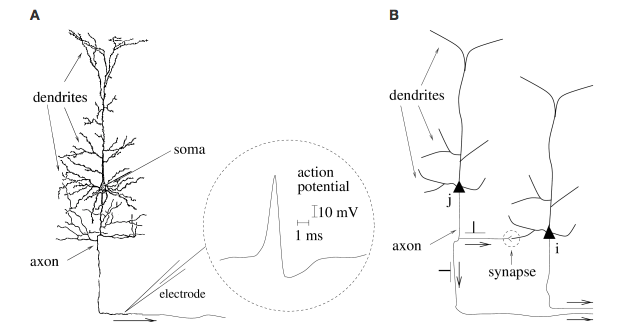
\includegraphics[scale=0.6]{images/neuron.png}
\caption[Neuron Morphology]{\textbf{A}. A cortical pyramidal cell with its soma, axon and dendrites highlighted. \textbf{B}. Signal transmission from neuron $j$ (presynaptic cell) to neuron $i$ (postsynaptic cell). Reproduced from \cite{Gerstner:2014}.}
\label{fig:neuron_morphology}
\end{figure}

A neuron spikes when the current input carried by the dendrites exceeds a certain threshold. The biochemical details of this process are not relevant for this project and the variety in electrophysiological properties of neurons \cite{Llinas:2008} leads to necessary simplification in order to simulate them. The signals emitted by neurons are called action potentials or spikes, and an approximate form is shown in the circled area of  \cref{fig:neuron_morphology}. A key property of action potential is that the form does not carry any information, information is actually carried by the number of action potentials and their timings \cite{Gerstner:2014}. After each spike the neuron enters a state called refractory period, in which it is impossible for it to spike again.  

Several mathematical models are available in order to simulate neurons, the one used in this project is a leaky integrate-and-fire (LIF) neuron model. 

% TODO insert maths details of LIF model

\subsection{Spiking Neural Networks}
Spiking neural networks are artificial neural networks which are closer to biology than the one commonly used nowadays for machine learning tasks. In spiking neural networks the concept of time is introduced and the communication between neurons relies exclusively on discrete spikes, the ones described in the previous section, instead of continuous values. 

The field of spiking neural networks is still in its infancy and lacks an effective supervised method for training, the equivalent of backpropagation for artificial neural network.


\section{SpiNNaker}
In order to handle the obvious complexity of neural simulation two approaches are possible. The first one is to use supercomputer built for general purpose task like in the case of the Blue Brain project which uses IBM's Blue Gene supercomputers \cite{Markram2006}. The second approach is to employ neuromorphic systems. These systems are designed around the idea that small computing elements (the ``neurons'') perform computation in a highly distributed manner in ways that mimic biological brains \cite{Furber2016}. Several of these systems have been developed recently, for example IBM TrueNorth, Stanford Neurogrid and University of Manchester SpiNNaker, which will be the system used for this project.

SpiNNaker is a massively-parallel multi-core computing system designed for large scale brain simulations running in biological real time. The system had been designed focusing on scalability, in order to model the very large number of components in a biological brain, and energy efficiency.

\begin{figure}[ht]
\centering
\begin{subfigure}{0.45\textwidth}
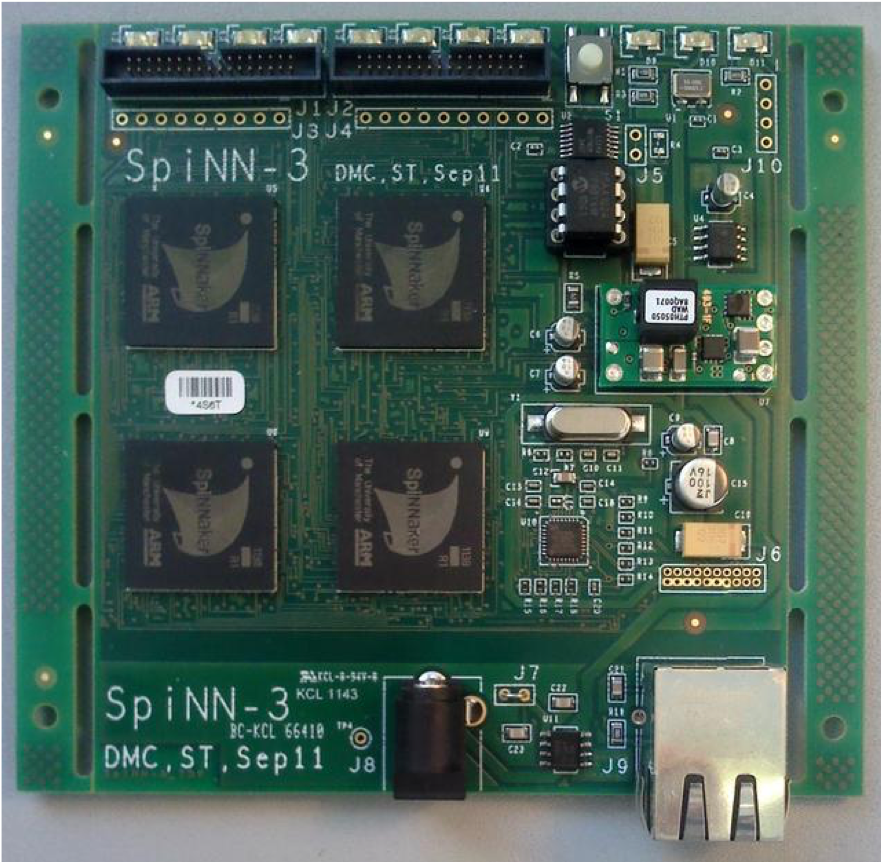
\includegraphics[width=\textwidth]{images/spinnaker_board.png} 
\caption{SpiNNaker board with 4 chips.}
\label{fig:spinnaker_board}
\imagesource{http://apt.cs.manchester.ac.uk/projects/SpiNNaker/hardware/index3.php}
\end{subfigure}
\begin{subfigure}{0.45\textwidth}
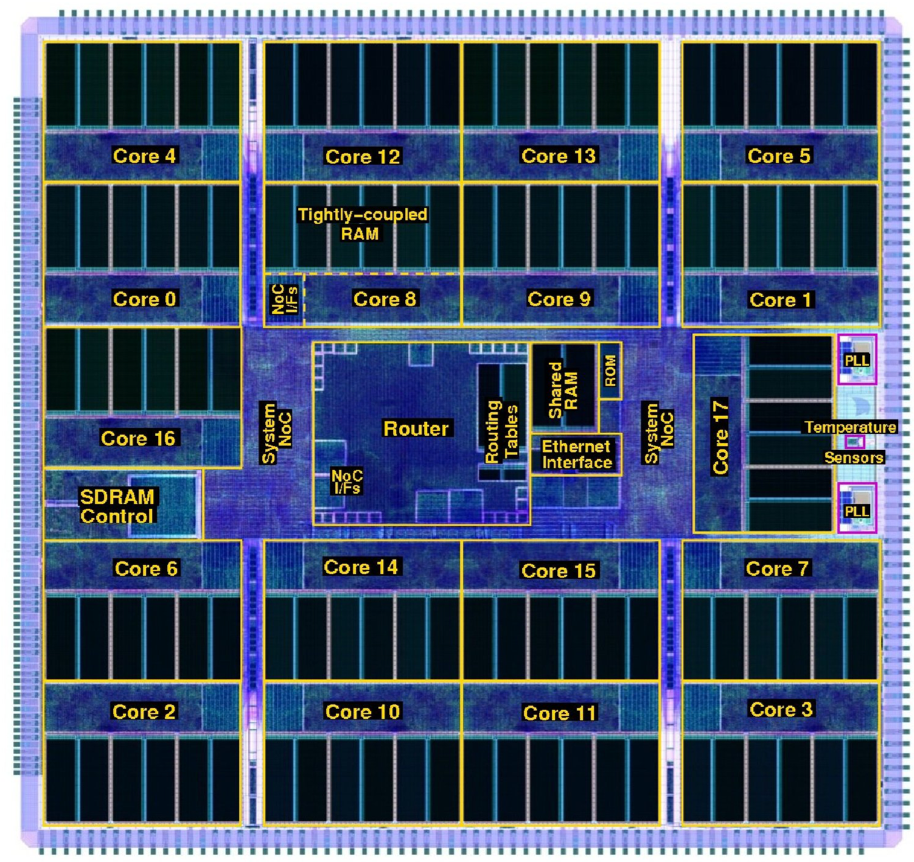
\includegraphics[width=\textwidth]{images/spinnaker_chip.png}
\caption{SpiNNaker chip}
\label{fig:spinnaker_chip}
\imagesource{http://apt.cs.manchester.ac.uk/projects/SpiNNaker/SpiNNchip}
\end{subfigure}
\caption[SpiNNaker Board and Chip]{SpiNNaker board and chip}
\label{fig:spinnaker}
\end{figure}

SpiNNaker is available at different scale, from a 4 chips board shown in \cref{fig:spinnaker_board} to a 1,036,800 cores machine accessible through the Neuromorphic Computing platform of the Human Brain Project \footnote{\url{https://www.humanbrainproject.eu/en/silicon-brains/} --- Accessed 19 April 2019}.

For this project, a 4 chips board has been used. Each chip, \cref{fig:spinnaker_chip} includes 18 ARM9 cores and \SI{128}{\mega\byte} of SDRAM. The board is connected to a host machine through an Ethernet cable and it is powered through a \SI{5}{\volt} \SI{1}{\ampere} USB cable.


\section{Dynamic Vision Sensor}
Due to the biologically inspired nature of this project and of the technologies involved, it made sense to use a Dynamic Vision Sensor as the input to the spiking neural network. A Dynamic Vision Sensor, also known as digital retina, is a device that records relative intensity changes for each individual pixel in continuous time.

\section{Motivation}


\section{Previous Work}

\label{sec:context}
\newpage

\chapter{Development}
\label{sec:development}
This chapter will first introduce PyNN, an high level language based on Python used to implement spiking neural networks, and then will describe the network in detail.

\section{PyNN}
PyNN is a Python library which defines a high level interface to create spiking neural networks in a simulator-agnostic fashion \cite{Davison2008}. Once a network is defined using PyNN, it can then be run on several available simulator like NEST, NEURON and Brian and different neuromorphic platforms, like SpiNNaker. In order to run PyNN defined scripts on SpiNNaker, sPyNNaker has been developed by the SpiNNaker group at the University of Manchester \cite{Rhodes2018}.

\begin{figure}[ht]
\centering
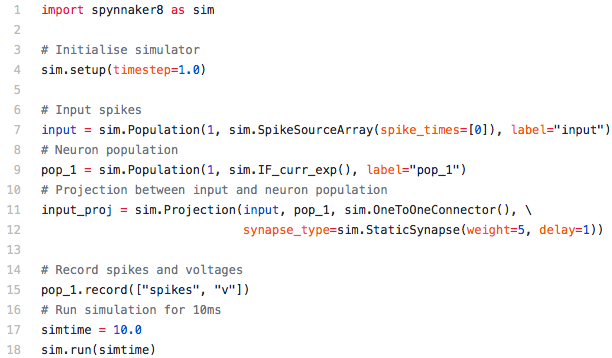
\includegraphics[scale=0.5]{images/development/pynn_example.png}
\caption[PyNN Example]{PyNN code example.}
\label{fig:pynn_example}
\end{figure}

PyNN defines spiking neural networks in terms of neurons grouped together in \emph{populations}. These populations are linked together using \emph{projections}. These projections use connection algorithms which can be selected from built-in methods or be explicitly defined. Parameters of the populations, like spike trains or voltages, can be recorded during the simulation and can be accessed when it is finished for further analysis. A brief code example is provided in \cref{fig:pynn_example}. 

\section{Shape Tracking Spiking Neural Network}
The network developed for this project draws its inspiration from the HMAX model proposed by Riesenhuber and Poggio \cite{Riesenhuber1999}. This model builds a hierarchy of increasingly complex representation in order to perform edge detection. An overview is shown in \cref{fig:hmax}. The \textsc{S1} and \textsc{C1} cells are part of the primary visual cortex V1.  

\begin{figure}[ht]
\centering
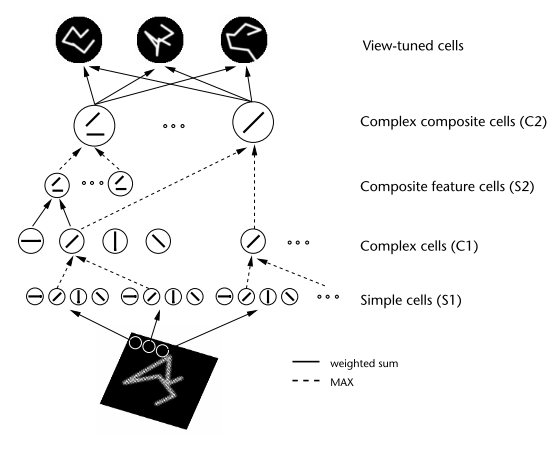
\includegraphics[scale=0.4]{images/development/hmax.png}
\caption[HMAX Model]{The HMAX model by Riesenhuber and Poggio \cite{Riesenhuber1999}.}
\label{fig:hmax}
\end{figure}

This model carries out edge detection alternating two main types of cells: simple cells \textsc{S} performing Gaussian-like tuning operations and complex cells \textsc{C} performing max operations. The \textsc{S} cells are of particular interest: they act as simple edge detector for the 4 main orientation of a line (horizontal, vertical, right diagonal and left diagonal) and they can be combined in order to obtain a desired shape. The \textsc{C} cells, with their max operation provide translation invariance and they are not useful for tracking shapes moving in a video stream.

\begin{figure}[ht]
\centering
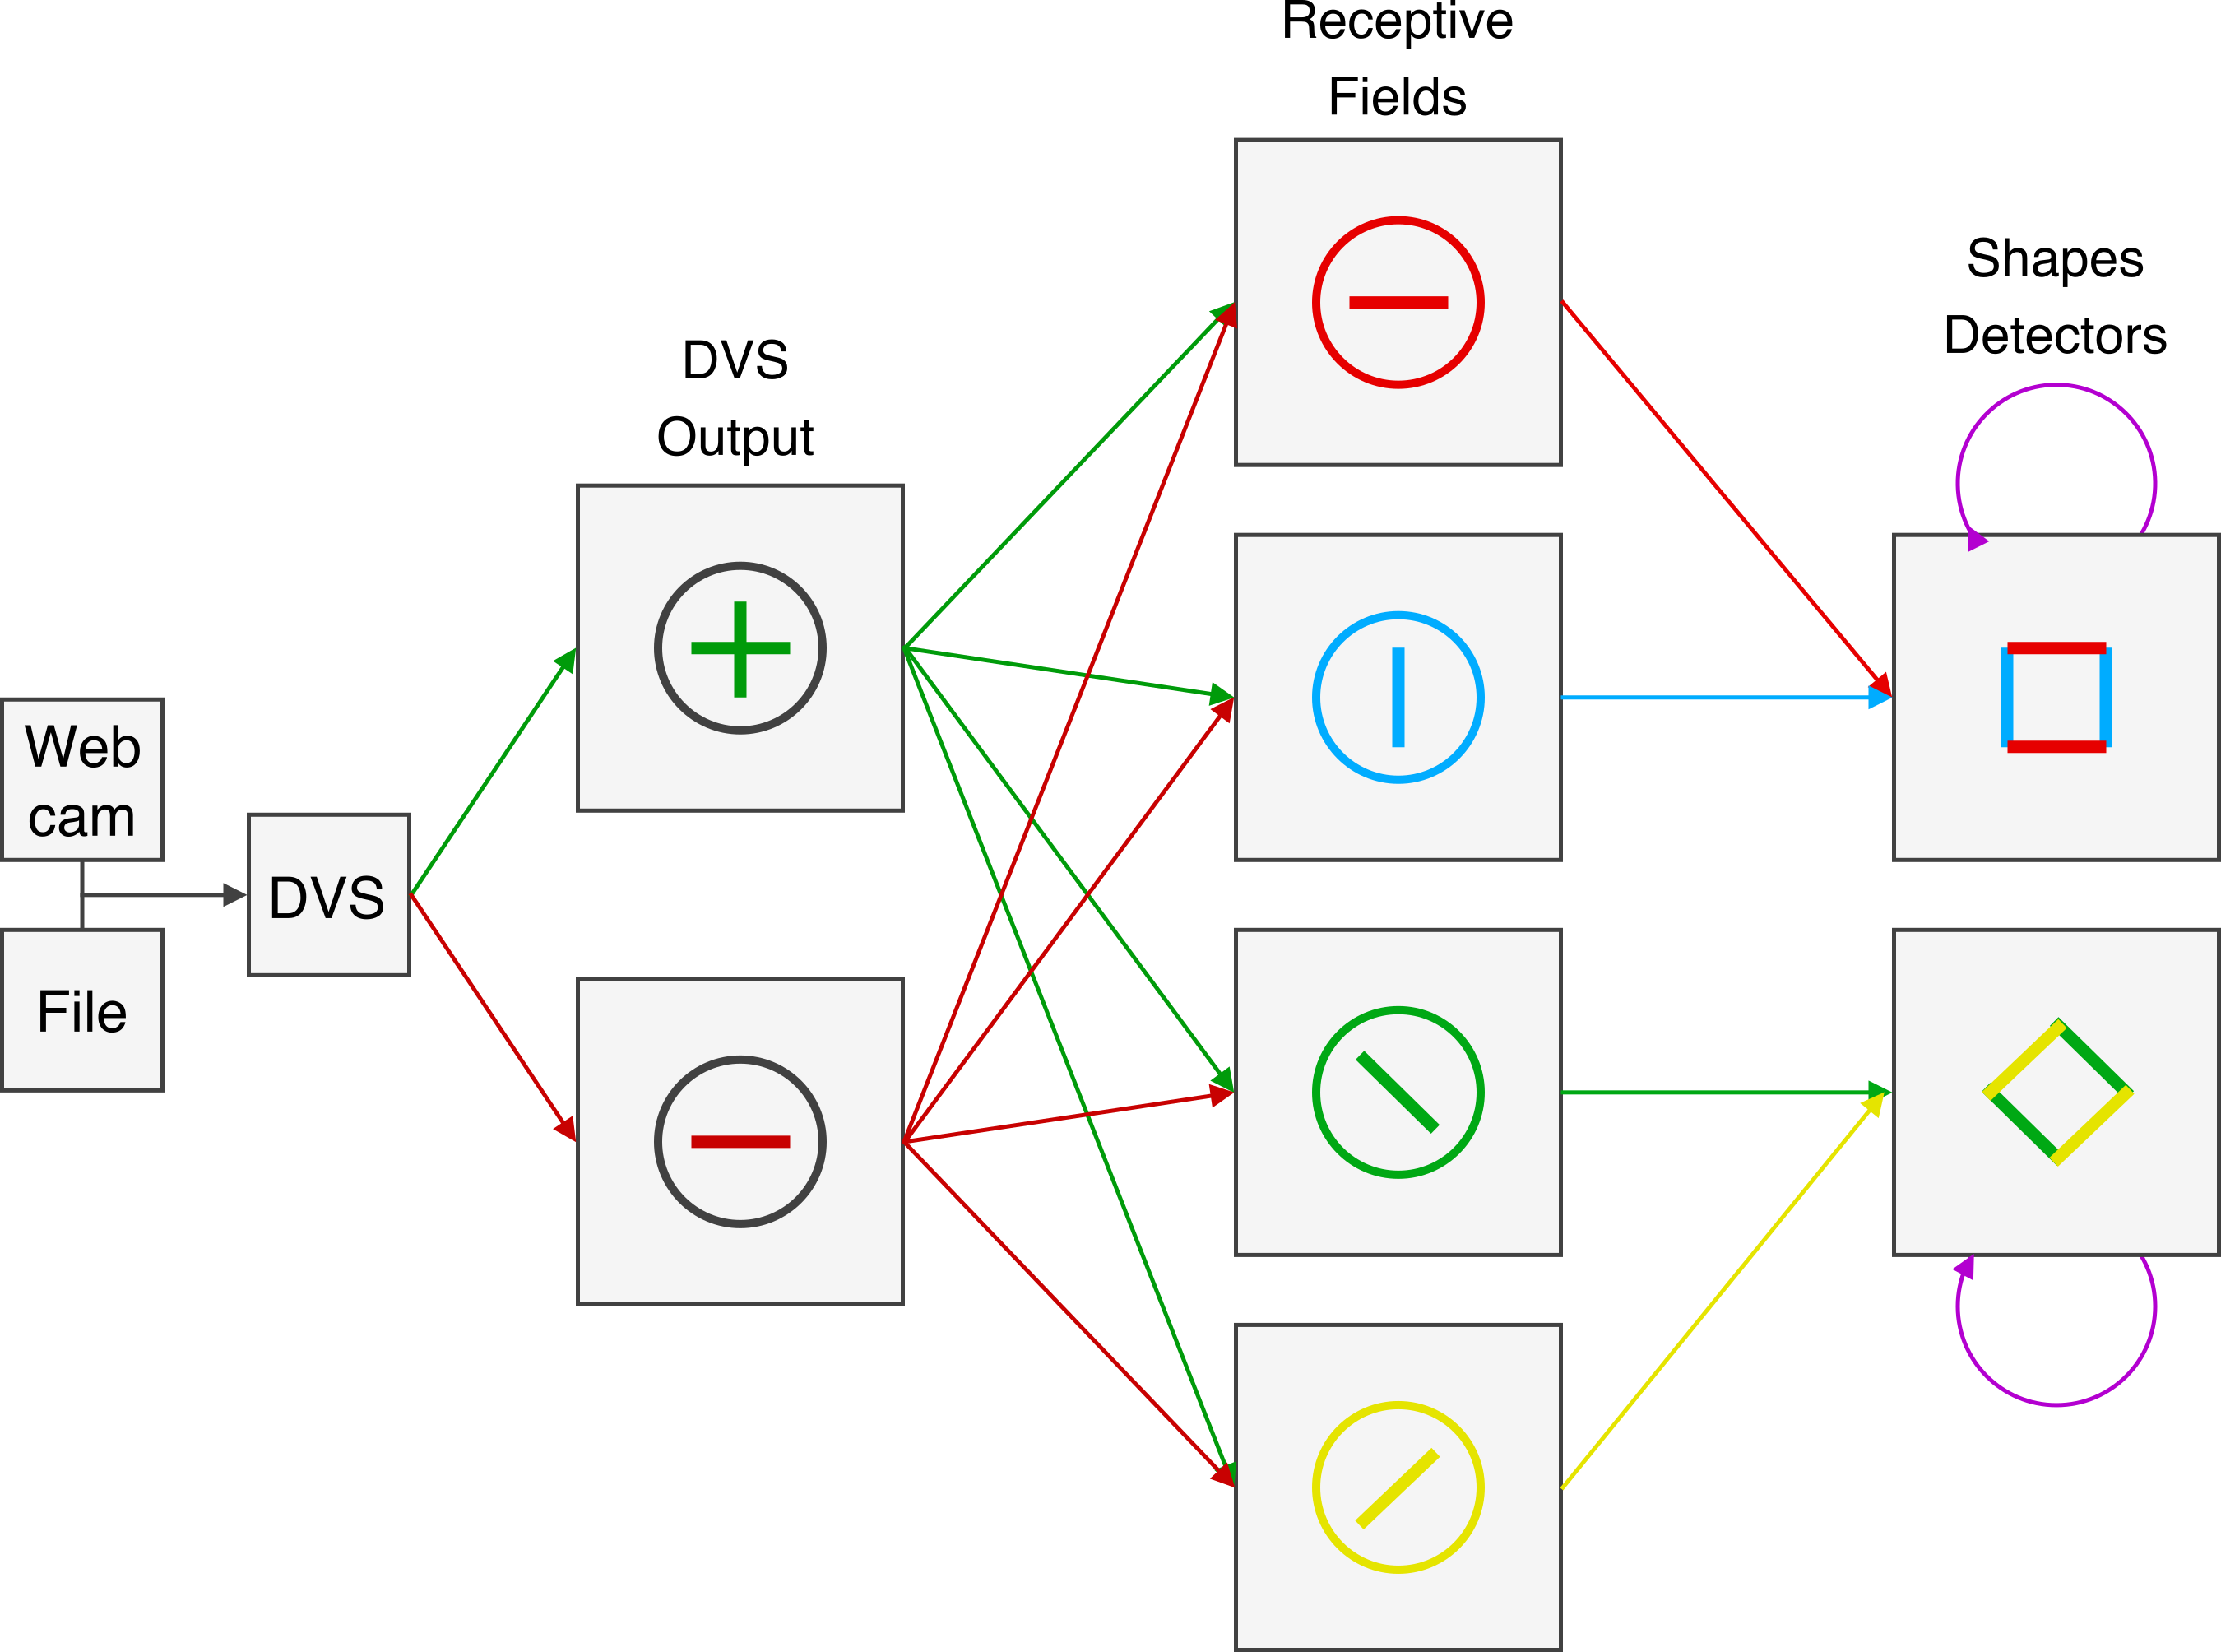
\includegraphics[width=0.75\textwidth]{images/development/network.png}
\caption[Network Overview]{The network developed for this project. The squares represent neuron populations, the arrows are the connections between populations.}
\label{fig:network}
\end{figure}

Based on these ideas, the network used in this project had been designed. A diagram is provided in \cref{fig:network}. The network is composed of 8 neuron populations, each comprising  $32 \times 32 = 1024$ LIF neurons, divided in 3 ``layers'': the DVS outputs, the receptive fields and the shapes detectors. The input of the DVS has a spatial of resolution $32 \times 32$ pixels and it could be either a prerecorded video or a live recording using a webcam. This allows the neurons to have a one-to-one mapping with the pixels in the input video. 

\subsection{DVS Emulator Output}
The DVS emulator produces two separate spikes streams, one for positive changes in pixel brightness (the green ones in \cref{fig:network}) and one for negative ones (the red ones). These spikes are injected into the network using two \texttt{SpikeSourceArray}, a PyNN object which emits spikes at specific times and can be treated in a similr way to a normal neuron population. The input of a \texttt{SpikeSourceArray} is a list of times for each neuron in the population. 

\begin{figure}[ht]
\centering
\begin{subfigure}{0.45\textwidth}
\centering
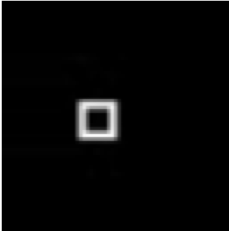
\includegraphics[width=0.5\textwidth]{images/development/dvs_square_lr.png} 
\caption{Screenshot of a video of a white square moving on a black background from left to right}
\label{fig:dvs_square_lr}
\end{subfigure}
\begin{subfigure}{0.45\textwidth}
\centering
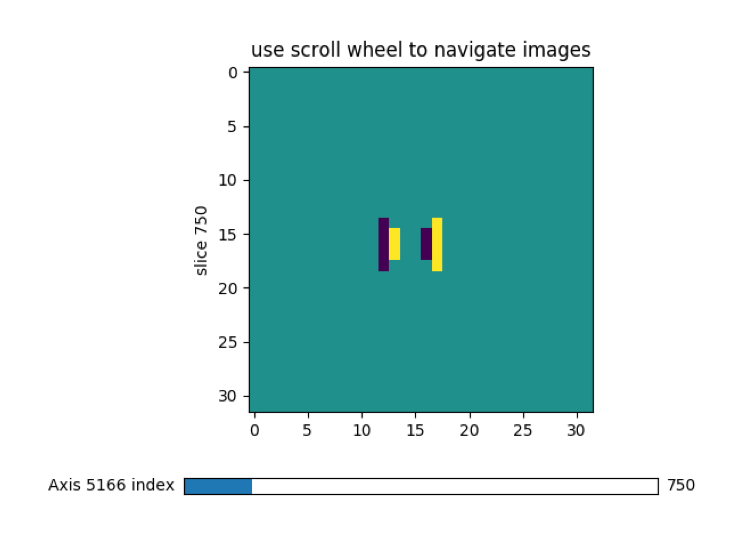
\includegraphics[width=\textwidth]{images/development/spikes_square_lr.png}
\caption{DVS output of the same square moving from left to right. In yellow the positive spikes and in purple the negative ones.}
\label{fig:spikes_square_lr}
\end{subfigure}
\caption[DVS Output of a Square]{Screenshot and DVS output of a square moving from left to right on the screen.}
\label{fig:square_lr}
\end{figure}

In \cref{fig:square_lr}, a \SI{5}{s} video of a white square moving from left to right is shown. This video has been synthetically generated using a Python script. The DVS emits spikes only on the horizontal edges and on the first pixel of the top and bottom edges. This is due to the fact that on the top edge (and the bottom one), the pixel brightness does not change apart from the rightmost and leftmost pixels.

\subsection{Receptive Fields}
In the context of the visual system, a receptive field is a region of the retina associated with a neuron which spikes when the region is stimulated by light. The neurons in this layer are the \textsc{S1} cells discussed previously. These forms 4 populations of cells, one for each of the 4 bar orientations (horizontal, veritcal and the two diagonals). 

The receptive fields are modelled upon the Octopus retina, as described by Folowosele in \cite{Folowosele2011}. An illustration is provided in \cref{fig:receptive_fields}.

\begin{figure}[ht]
\centering
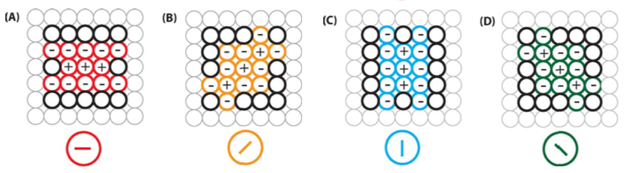
\includegraphics[scale=0.6]{images/development/receptive_fields.png}
\caption[Receptive Fields]{Illustration of the receptive fields of the \textsc{S1} cells implemented in the network. The $+$ represents excitatory connections, the $-$ represents inhibitory connections and the empty circles have no effects on \textsc{S1} cells.}
\label{fig:receptive_fields}
\end{figure}

The receptive fields are constructed using connections between the positive and negative polarities \texttt{SpikeSourceArray}s, the DVS output layer in \cref{fig:network}, and the 4 populations of \textsc{S1} cells. Each neuron in a \textsc{S1} cells population has 3 excitatory connections to the positive polarity \texttt{SpikeSourceArray} and 10 inhibitory connections to the negative polarity \texttt{SpikeSourceArray} accordingly to the patterns shown in the figure. For neurons close to the edges, only the connections falling inside the $32 \times 32$ frame are set.

An example of the behaviour of these populations of cells is shown in \cref{fig:receptive_fields_square_lr}.

\begin{figure}[ht]
\centering
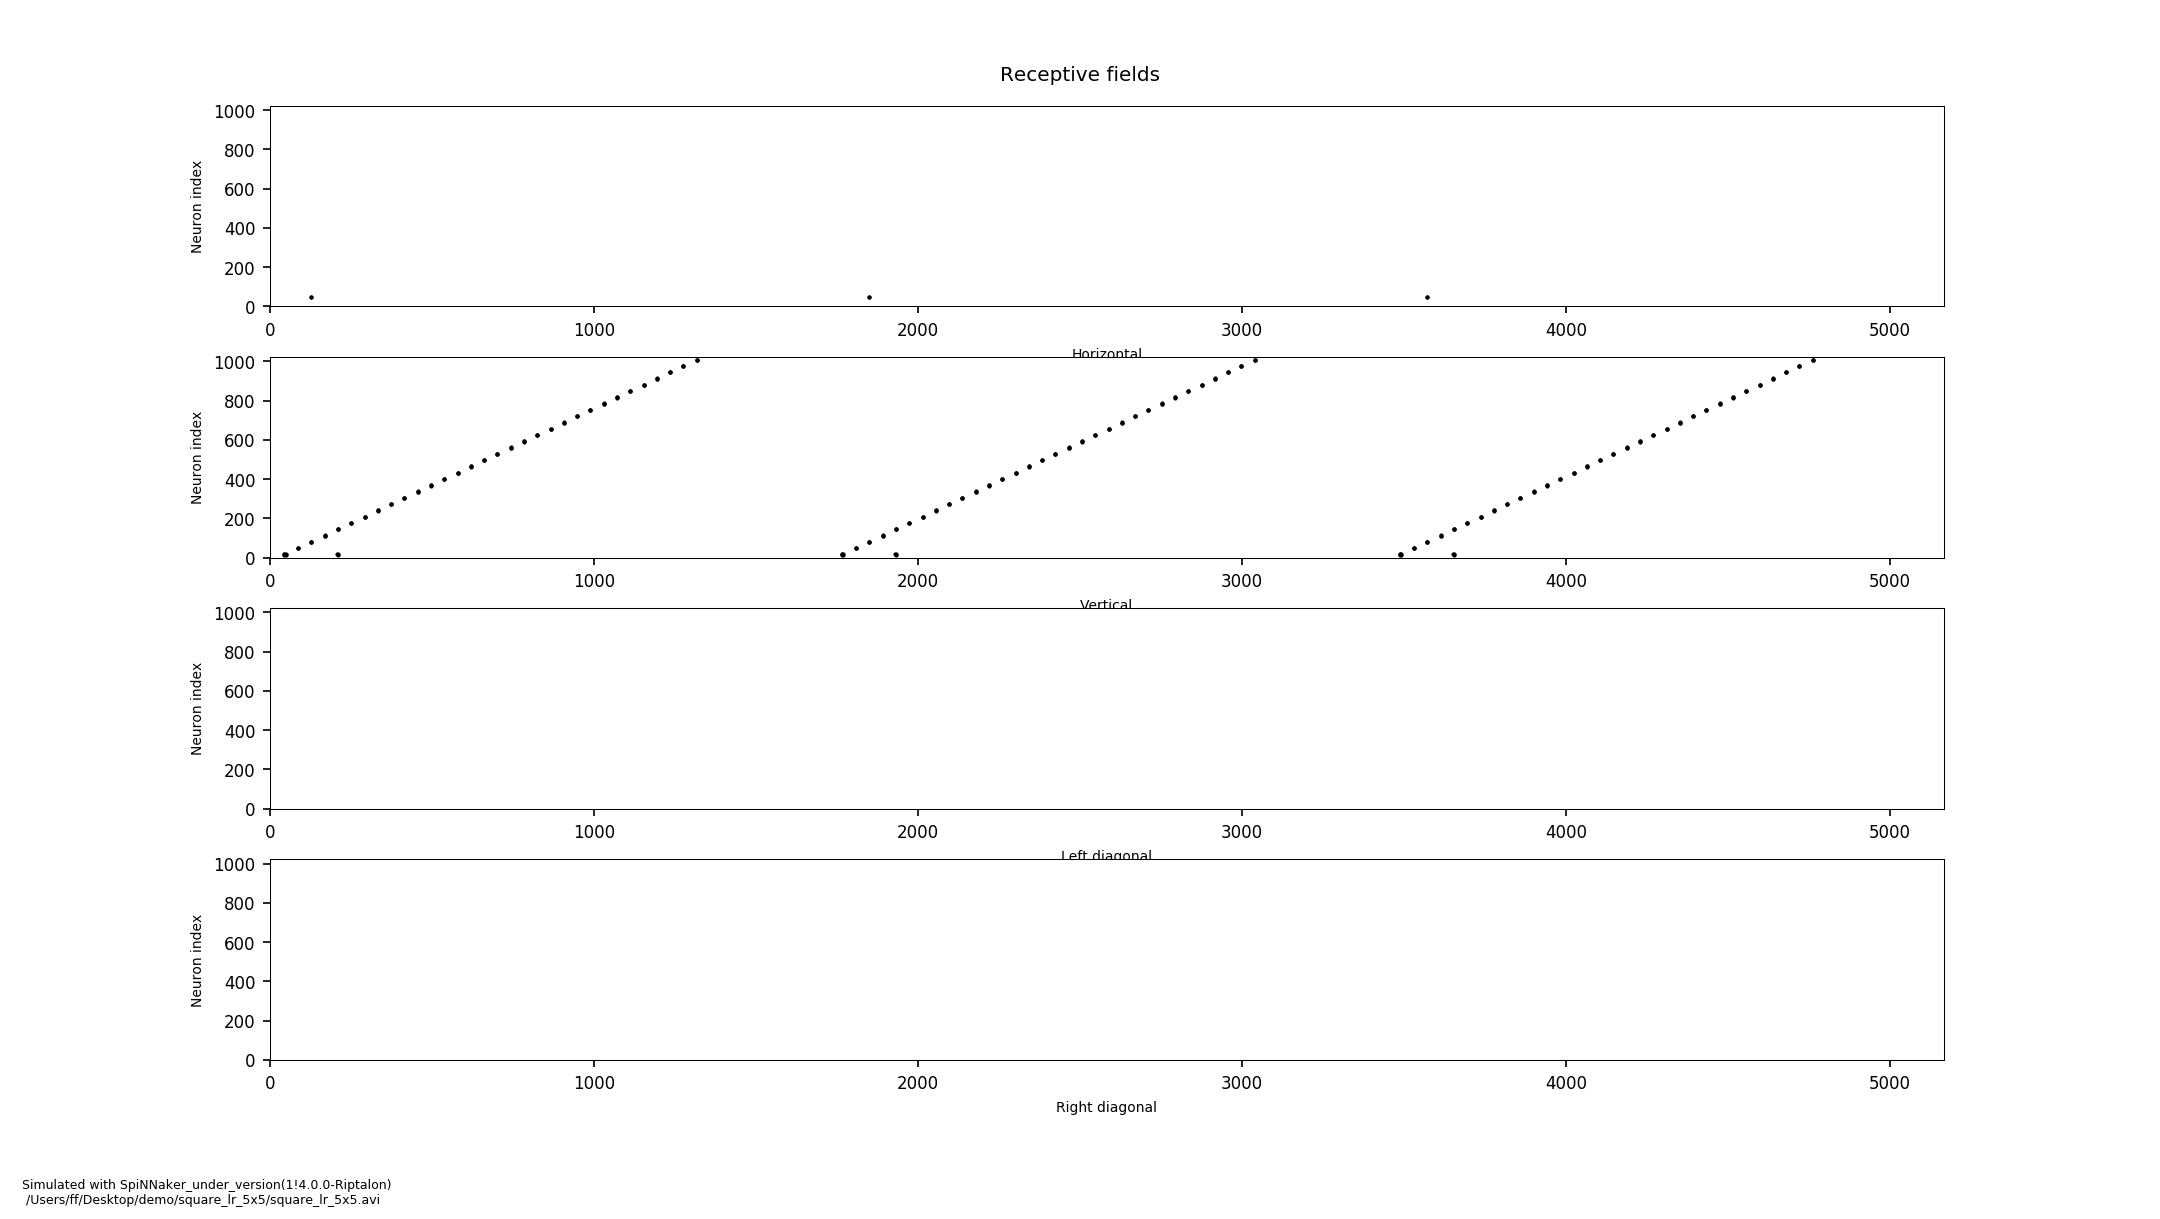
\includegraphics[width=\textwidth]{images/development/receptive_fields_square_lr.png}
\caption[Receptive Fields Spike Trains of Square]{Spike trains of the 4 population of cells when the video of the square moving from left to right is presented. From top to bottom: horizontal, vertical, left diagonal (green in \cref{fig:receptive_fields}) and right diagonal (yellow in \cref{fig:receptive_fields}). On the $x$ axis there is time in milliseconds, on the $y$ axis the neuron ids. In this example it can be seen that only vertical edges are found and some small noise on the horizontal ones due to the square entering the screen. Due to resolution constraints not all the spikes can be seen, a single dot comprises multiple spikes.}
\label{fig:receptive_fields_square_lr}
\end{figure}

\subsection{Shapes Detector}
Once the receptive fields had been set up, they can be combined in various way in order to create populations of cells able to detect shapes.

The network in its current form recognises only two shapes: a square and a diamond. For each shape a population of cells had been created.

The ``square detector'' combines horizontal and vertical edges in order to detect squares of size $5 \times 5$. On the other hand, the ``diamond detector'' combines the left and right diagonal edges to detect diamonds of size $5 \times 5$. 

\subsection{Shape Recognition}




\newpage

\chapter{Evaluation}
\label{sec:evaluation}
In this chapter, the approach to code testing and a discussion on the problem on how to evaluate the network performance will be presented.


\section{Code testing}
The codebase can be divided in three major components: the sPyNNaker code, the DVS emulator and the network written for the project. 

The sPyNNaker code is already heavily tested by its developers in the SpiNNaker group. The DVS emulator did not included any unit tests but none were added as part of this project due to time constraints. An extensive review of the code and hours of experiments convinced the author of this report that the emulator performed as expected.

Unit tests had been included in the code specifically written for this project. In particular, all the code that defines the connections between the DVS output and the receptive fields and between the receptive fields and the shapes detectors has unit tests. 

A continuous integration server had been set up using the free tier of \href{http://travis-ci.com}{travis-ci.com}, a continuous integration tools provider, in order to run all the unit tests at every git push. 


\section{Evaluation of the Network}
Evaluating the performances of this network is quite difficult. In particular, there is no labelled dataset on which the network has been trained. 
The videos used had been generated using a Python script and they cover quite simple and optimal scenarios. 

In order to make the experiments reproducible, the network runs using configuration files stored as YAML. Since these files are plaintext, they can be versioned in order to keep track of the changes. An example can be seen in \cref{fig:config_file}. 

\begin{figure}[ht]
\centering
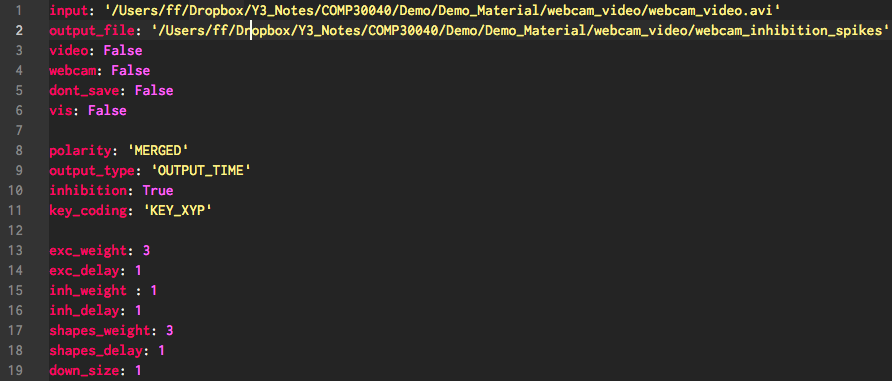
\includegraphics[width=\textwidth]{images/evaluation/config_file.png}
\caption[Config File for the Network]{An example config file is shown. Settings for the network can be changed and tracked across different experiments.}
\label{fig:config_file}
\end{figure}

The network performs very well with both squares and diamonds from synthetic videos. The problems with these videos is when the square is moving parallel to the edges of the frame (or the diamond diagonally) as these edges do not generate any spikes, like in the example shown in \cref{fig:square_lr}. 

On synthetic videos the networks is able to recognise quite well shapes of size $5 \times 5$ and $7 \times 7$, as long as their movements on the screen generate enough spikes, for example in the case of a square moving from the top left corner to the bottom right one. 

Another problem is when shapes do not move, hence they do not generate spikes. The human eyes do not look at a scene staying still, instead, they move around and these movements are called saccades. A way of simulating saccades for handling still scenes would definitely help to solve this problem. 
Using a webcam as the network input does not produce any meaningful results, as it can be seen in \cref{fig:webcam_results}. The receptive fields, \cref{fig:receptive_fields_webcam_input}, produce spikes in the areas where the shape is moving, but the shape detectors, \cref{fig:shape_webcam_input}, produce too many spikes so that a clear location of where the shape is cannot be obtained. 

Evaluation results are presented in \Cref{app:evaluation}.

\begin{figure}[ht]
\centering
\begin{subfigure}{0.45\textwidth}
\centering
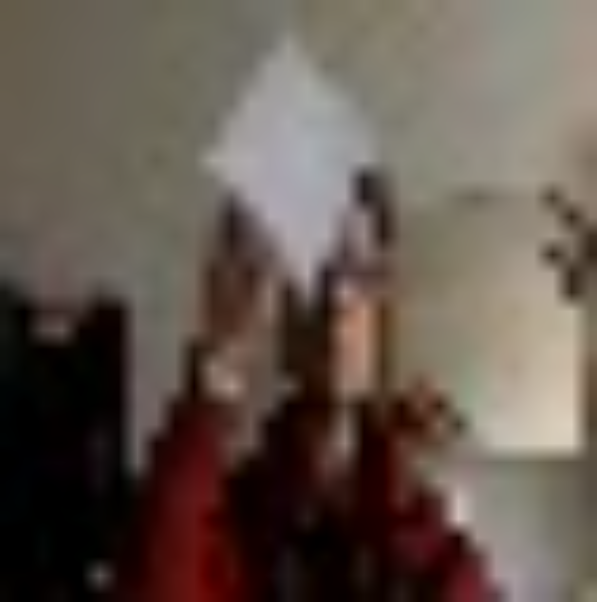
\includegraphics[width=0.5\textwidth]{images/evaluation/webcam_input.png} 
\caption{Screenshot of a recording of a webcam input for tracking the white diamond.}
\label{fig:webcam_input}
\end{subfigure}

\begin{subfigure}{\textwidth}
\centering
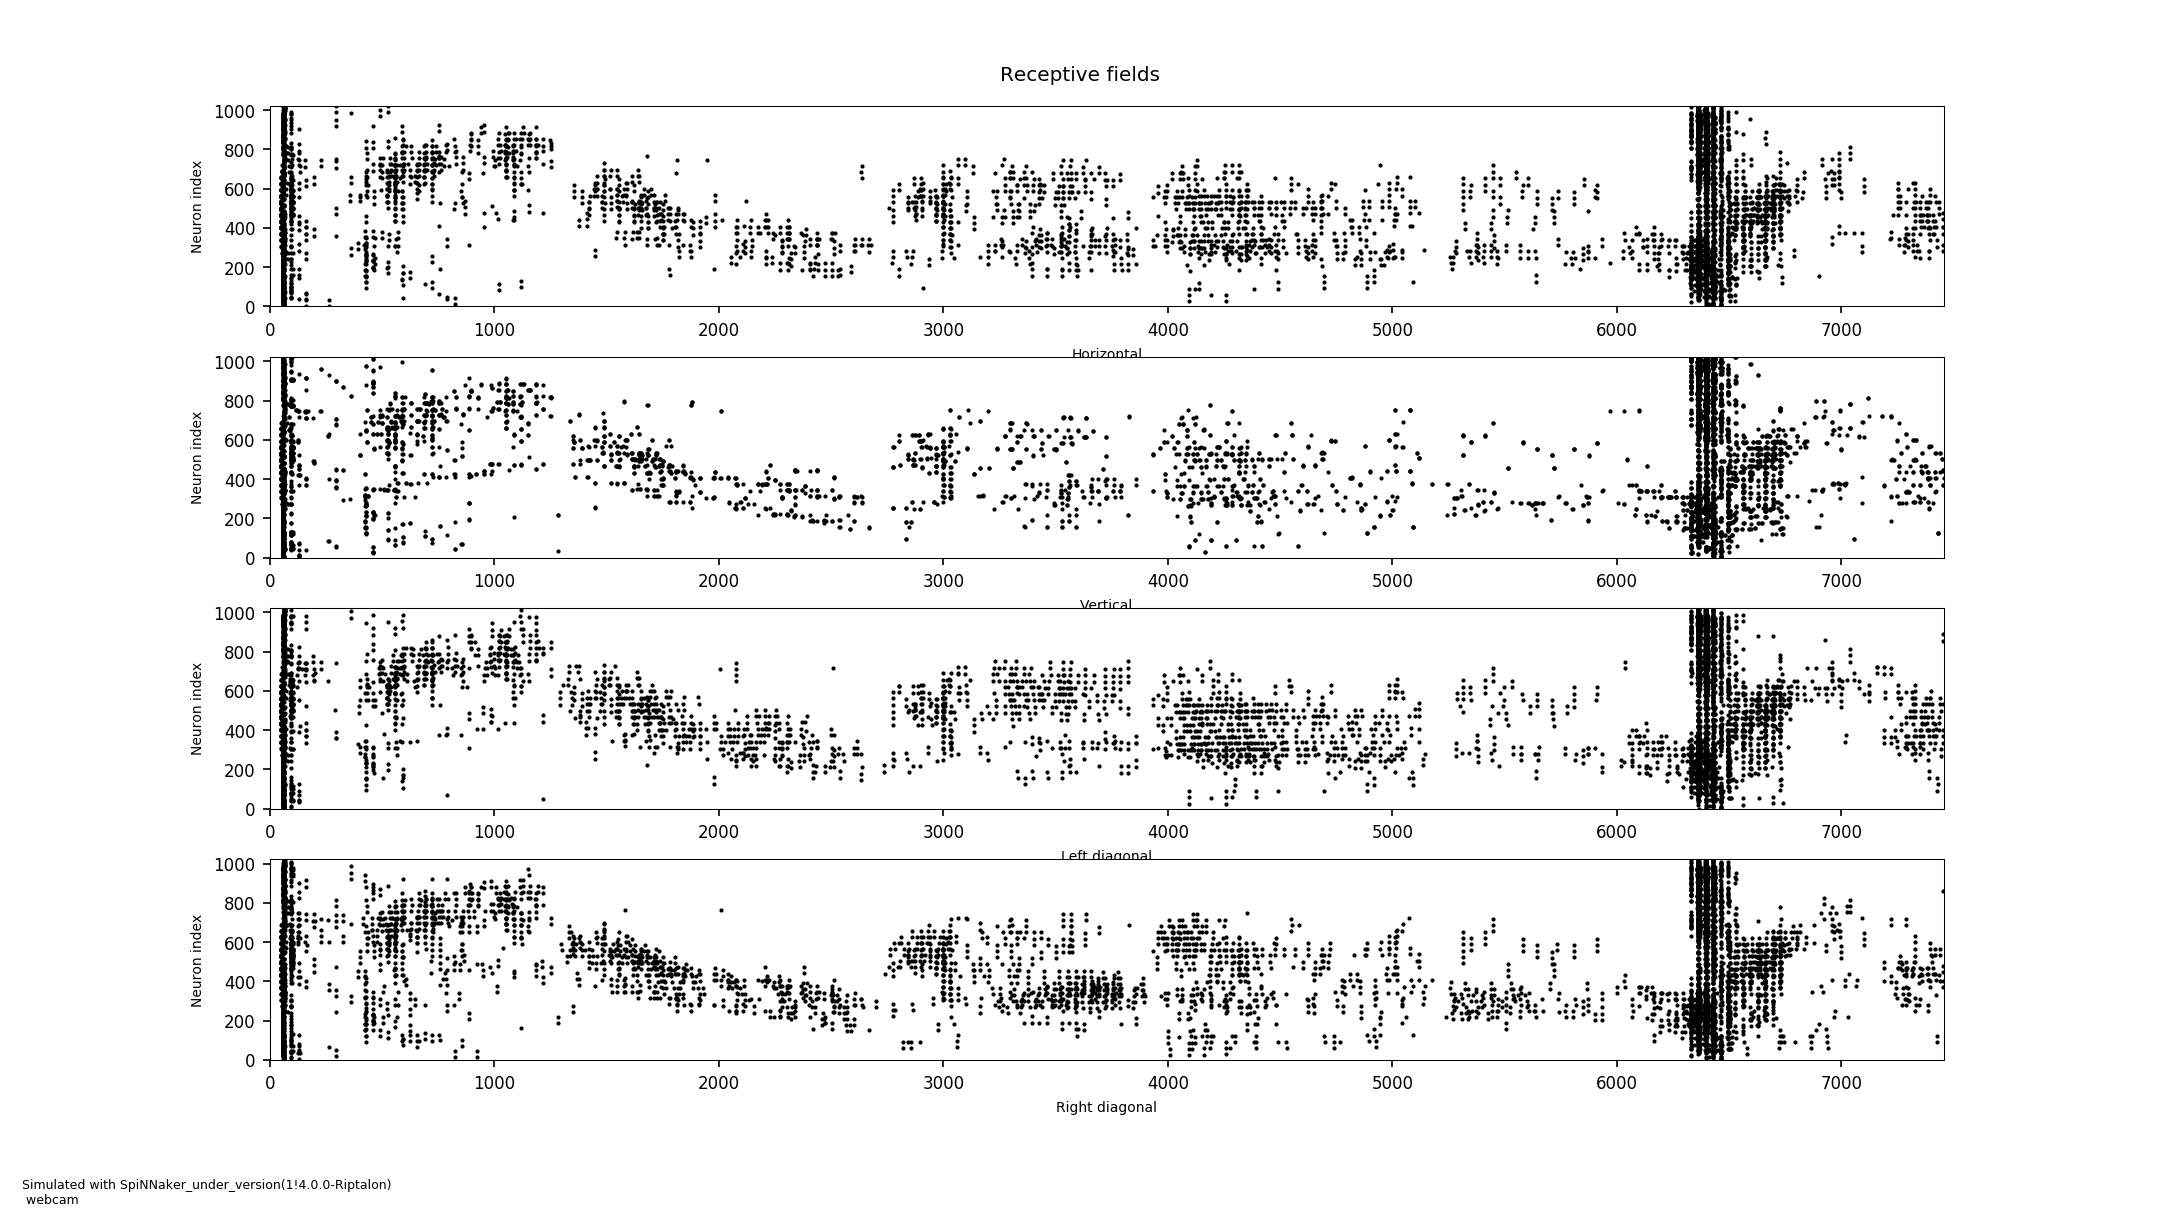
\includegraphics[width=0.75\textwidth]{images/evaluation/receptive_fields_webcam_input.png}
\caption{Edge detectors.}
\label{fig:receptive_fields_webcam_input}
\end{subfigure}

\begin{subfigure}{\textwidth}
\centering
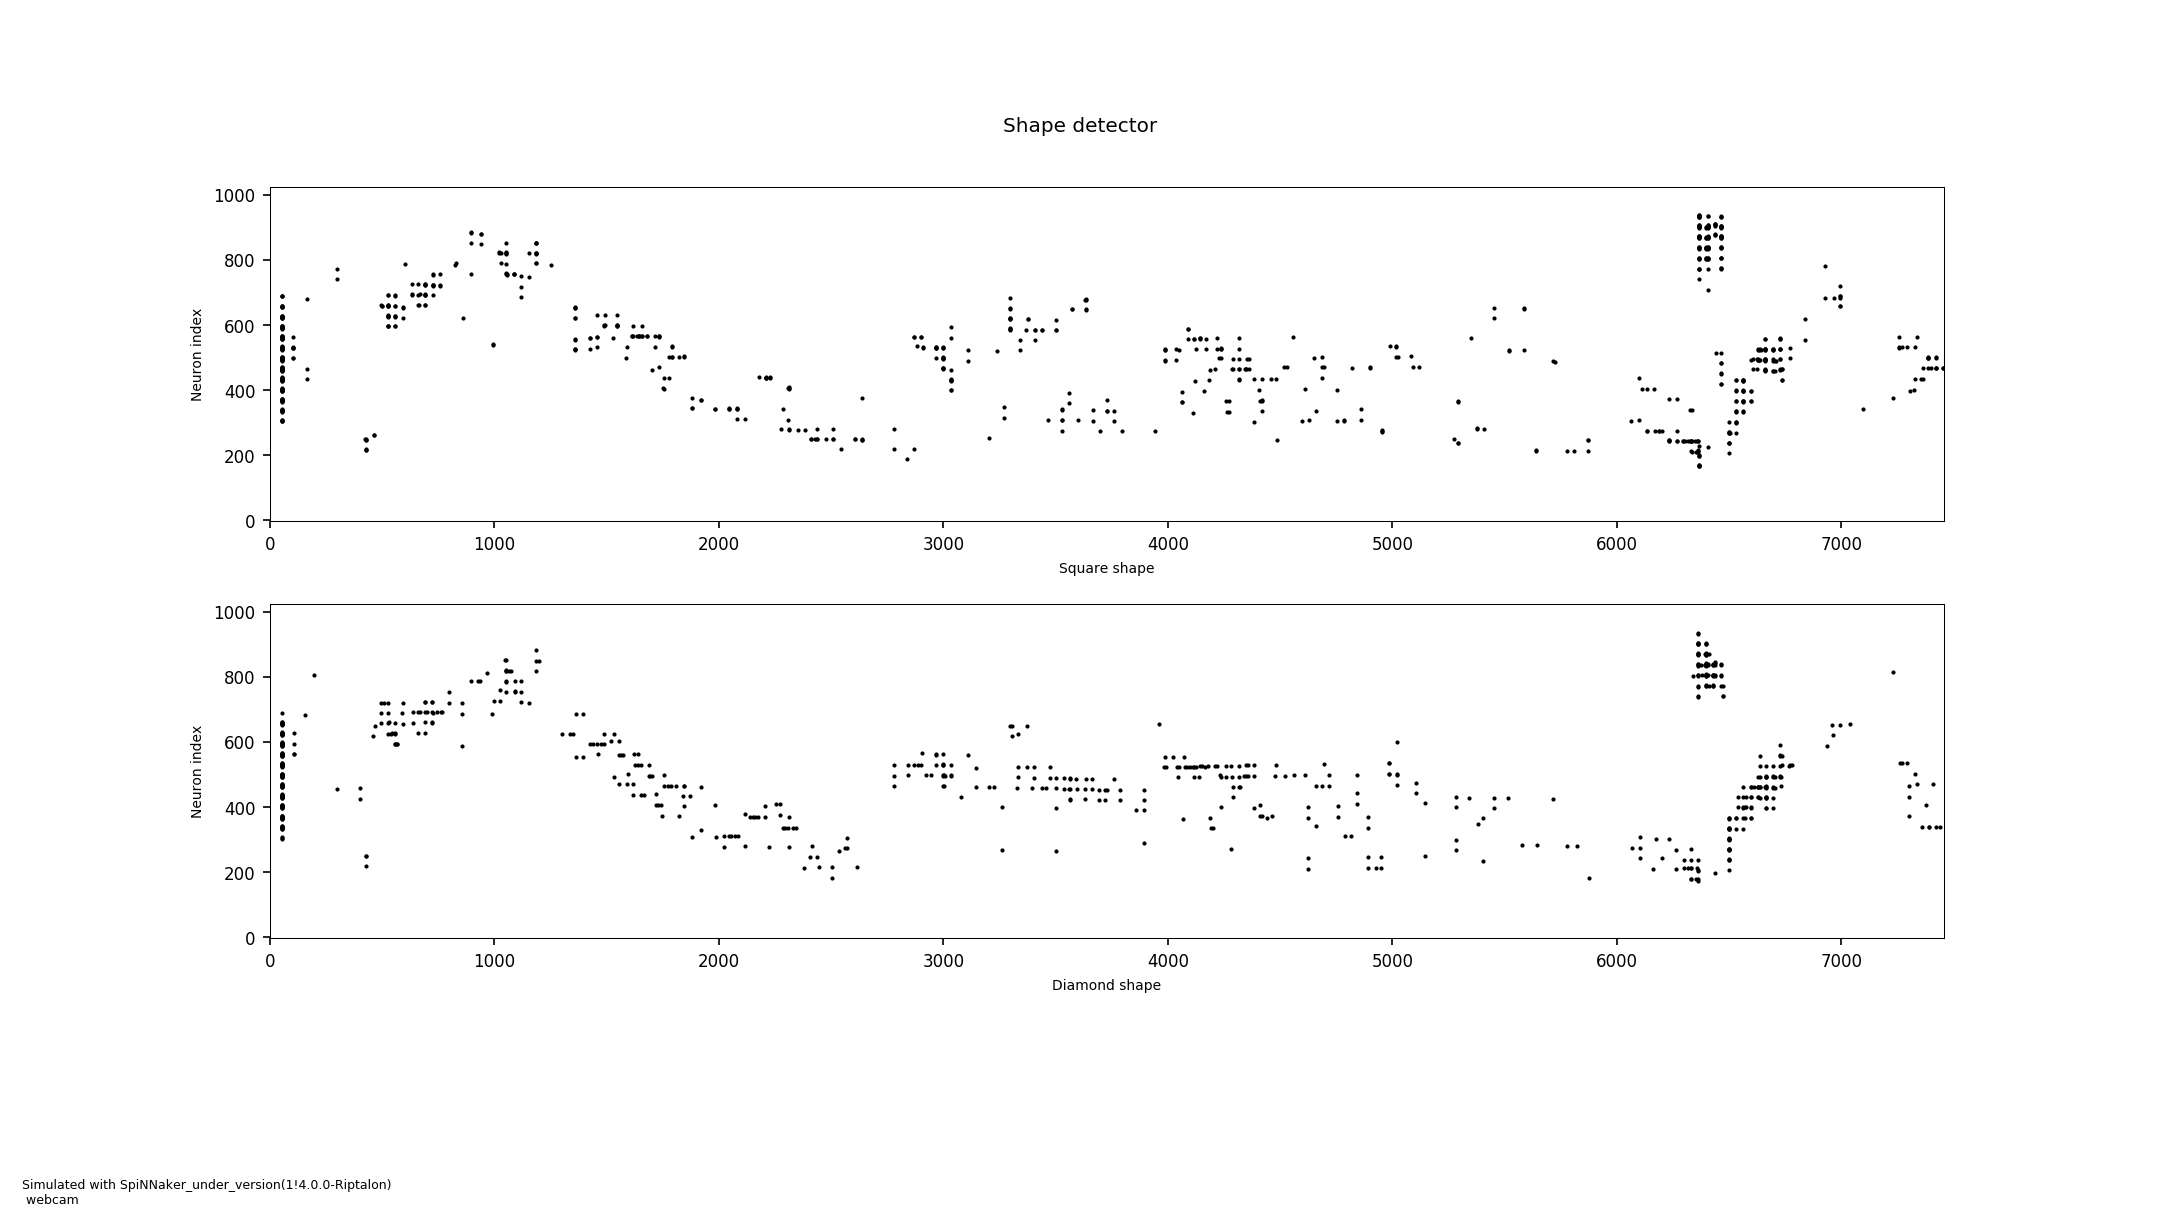
\includegraphics[width=0.75\textwidth]{images/evaluation/shape_webcam_input.png}
\caption{Shape detectors.}
\label{fig:shape_webcam_input}
\end{subfigure}

\caption[Webcam Input Results]{Screenshot and spike trains for the cells populations for a recording of a video registered with a webcam.}
\label{fig:webcam_results}
\end{figure}

\newpage

\chapter{Conclusion}
\label{sec:conclusion}
\section{New Knowledge}
The project required learning and understanding a lot of material which is not part of my degree. In particular, learning enough in order to understand the computational neuroscience literature required a great deal of effort and time. The lack of literature related to this specific task for spiking neural network was another obstacle which posed a great chance of failure. 

Luckily, Python was already known and only the PyNN API required to be learnt. 

\section{Project Development}
The project development run for 20 weeks, 12 in Semester 1 and 8 in Semester 2. The project presentation was planned to be between week 6 and 8 of Semester 2, so week 6 had been taken as the deadline for the actual development. Also, development stopped during Christmas for revision.

\begin{table}[ht]
\centering
\begin{tabular}{l|ll}
Milestones                    & Planned Weeks & Actual Weeks \\ \hline
Research                      & 1-4           & 1-6          \\
SpiNNaker Setup               & 1-4           & 1-3          \\
DVS Emulator Setup            & 5-8           & 4-8          \\
Receptive Fields Working      & 8-11          & 8-12         \\
Shapes using Synthetic Videos & 12-15         & 13-16        \\
Shapes using Webcam           & 15-18         & 16-19       
\end{tabular}
\caption{Milestones of the project and planned and actual weeks of development.}
\label{table:development}
\end{table}

\Cref{table:development} shows the main milestones of the project, how the development had been planned in September and how it went during the academic year.

A lot of time had been allocated for research and the initial setup. When devising the original plan, extra time had been added to each milestone. Retrospectively, this had been a good decision as it allowed the project to run pretty much on schedule throughout the year.

The biggest problem faced during the development was caused by an undetected bug in the code which sets the connections between cells populations. Due to this bug, getting the receptive fields to work as expected took longer than expected and added an extra week of development to the original plan. Other reasons causing delays were due to unreported incompatibilities in some of the libraries used during the 

\section{Reflection}
Overall, this project had been a great learning experience spanning different fields. 

Most of the planned milestones had been achieved. In particular, the network runs in real time on a 4 chips SpiNNaker board and achieves sensible results on the synthetic video.

Nevertheless, several limitations are still present. The network cannot be easily expanded in order to recognise new shapes: the connections have to be manually created for each new shape. Also, following the results shown in \cref{fig:shape_webcam_input}, the webcam input is too noisy for being useful. It is opinion of the author that in order to solve this problems, a deeper network, with populations of cells encoding higher levels of abstraction, could be used together with a learning algorithm like Spike Timing Dependent Plasticity (STDP) \cite{Song2000} in order to learn the connection weights between the cells populations. 
\newpage

\pagenumbering{roman}

\printbibliography[heading=bibintoc]

\appendix
\chapter{Evaluation Results}
\label{app:evaluation}
In this appendix, evaluation results for several of the synthetic videos are presented. 

In \cref{fig:square_lr_ev} it can be seen how the square moving parallel to two of its edges does not produces spikes for those edges. Only the vertical edge detector spikes in this case, \cref{fig:square_lr_receptive_fields}, and the shapes detector are unable to detect any shape in the visual field, \cref{fig:square_lr_shape}.

In \cref{fig:random_ev} the square and the diamond appear at a certain random location, stay still for about \SIrange{40}{80}{\milli\second} and then disappear and appear in a different location. The edge detectors are spiking only when the shapes change position, \cref{fig:random_receptive_fields}. Consequently, the shapes detectors spike at the same time, but in this case they provide an accurate tracking of the shapes, correctly differentiating between them, \cref{fig:random_shape}.

In \cref{fig:square_diag_ev} the square is moving diagonally from the top left corner to the bottom right one. The direction in which it moves, produces spikes for all edges, as it can be seen in \cref{fig:square_diag_receptive_fields} where both the vertical and horizontal detectors are spiking as expected. The tracking of the square is extremely accurate, as seen in \cref{fig:square_diag_shape}, with some noise due to the square entering the frame. 

%%%%%%%%%%%%%%%%%%%
\begin{figure}[ht]
\centering

\begin{subfigure}{\textwidth}
\centering
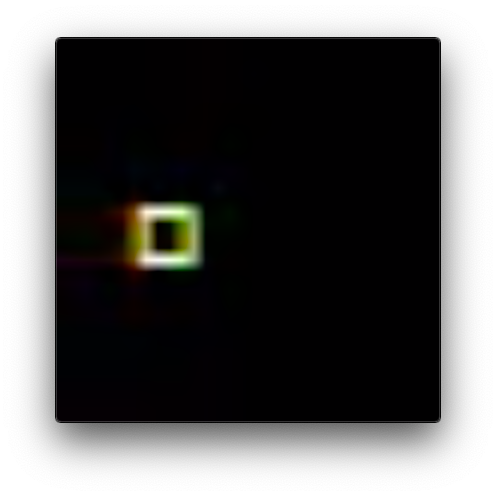
\includegraphics[width=0.3\textwidth]{images/appendix_evaluation/square_lr_spikes.png}
\caption{DVS emulator spikes superimposed over a frame of the video.}
\label{fig:square_lr_spikes}
\end{subfigure}

\begin{subfigure}{\textwidth}
\centering
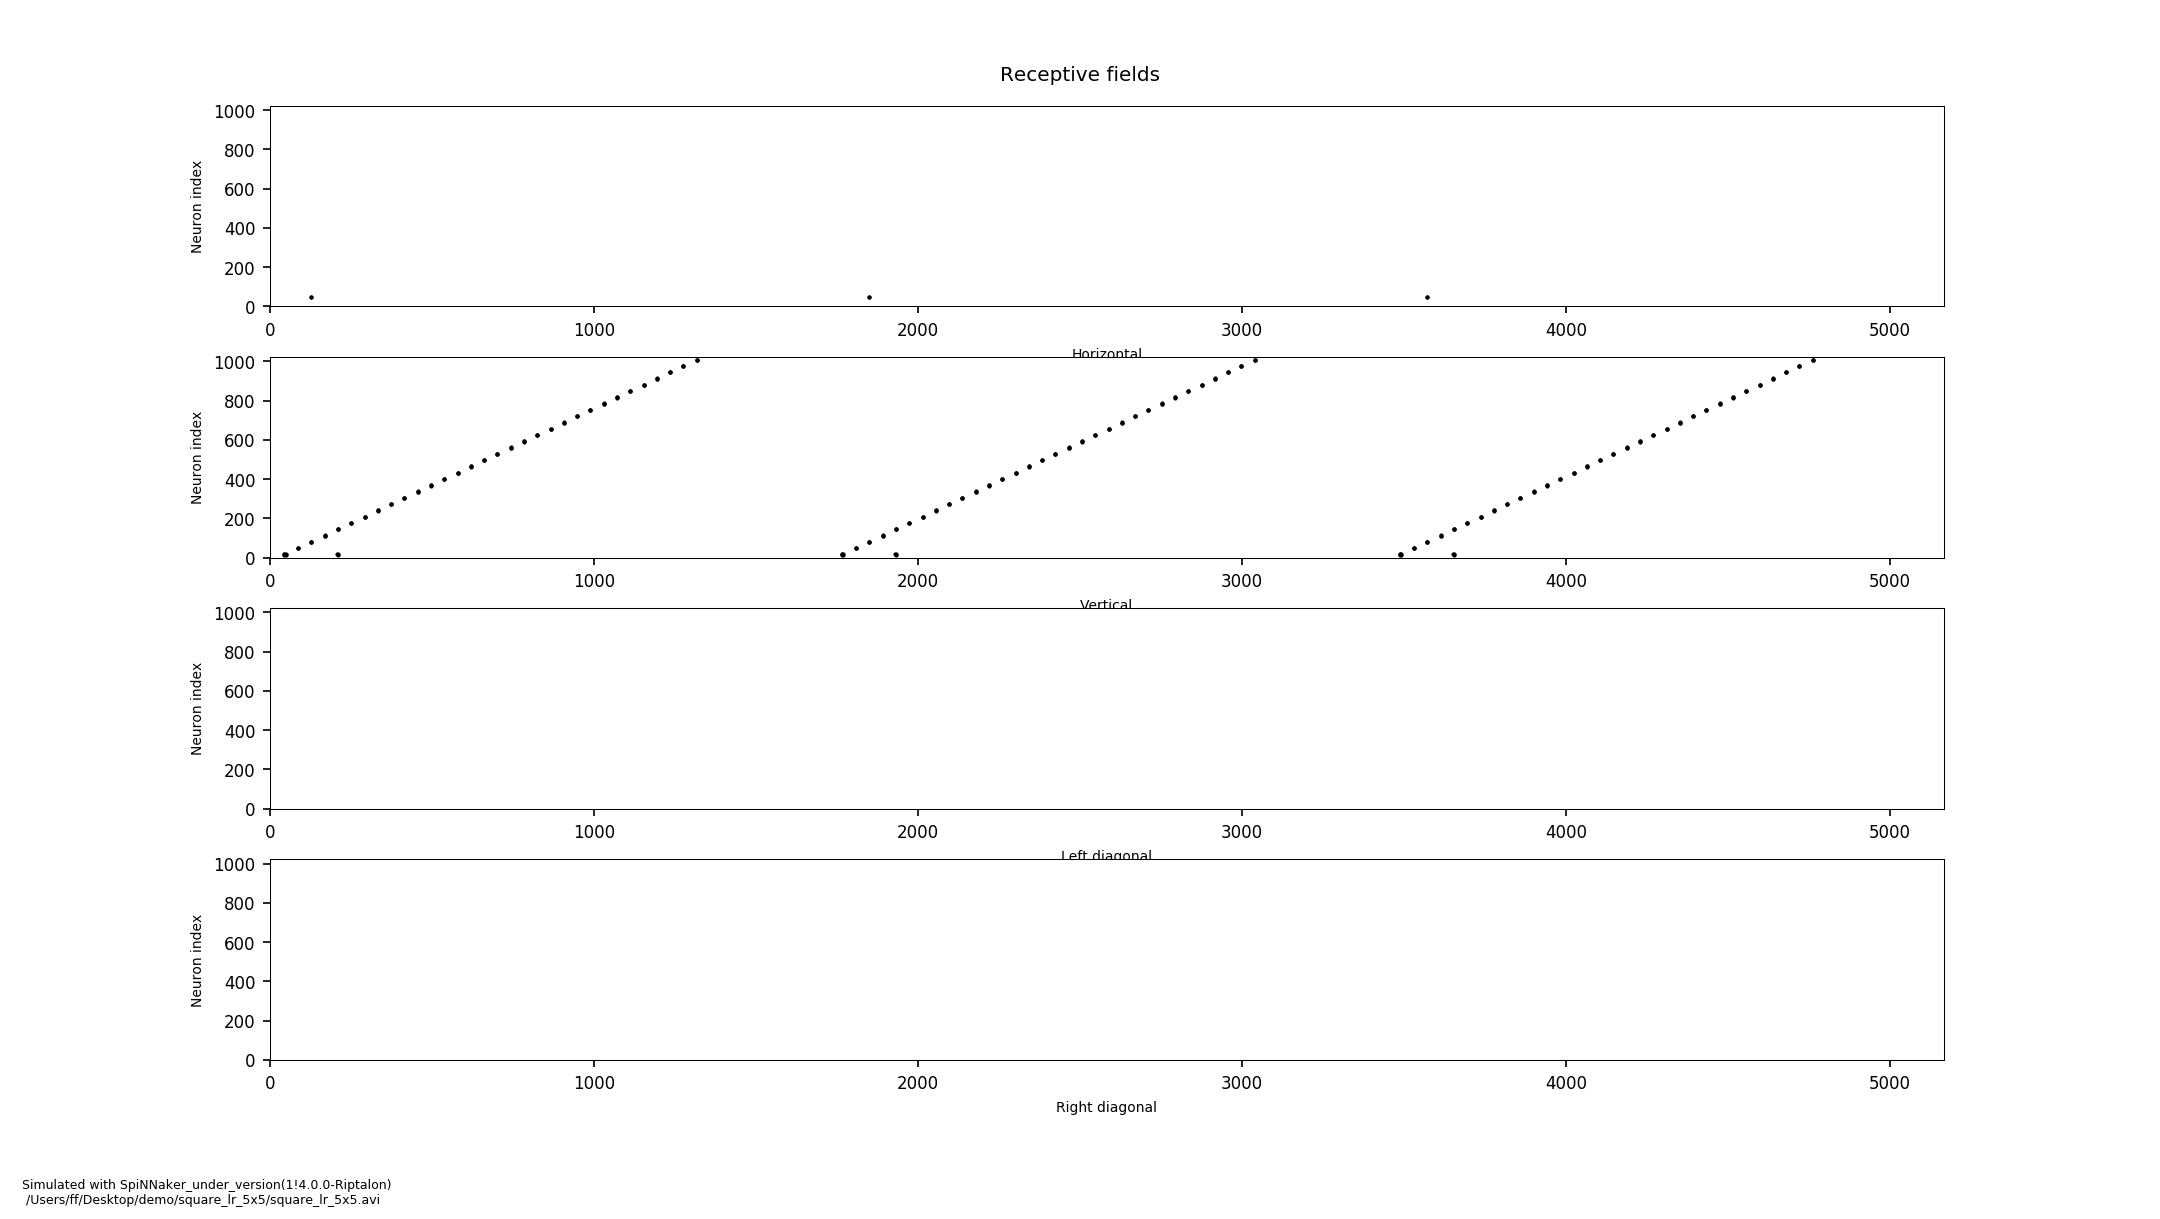
\includegraphics[width=0.75\textwidth]{images/appendix_evaluation/square_lr_receptive_fields.png} 
\caption{Edge detectors.}
\label{fig:square_lr_receptive_fields}
\end{subfigure}

\begin{subfigure}{\textwidth}
\centering
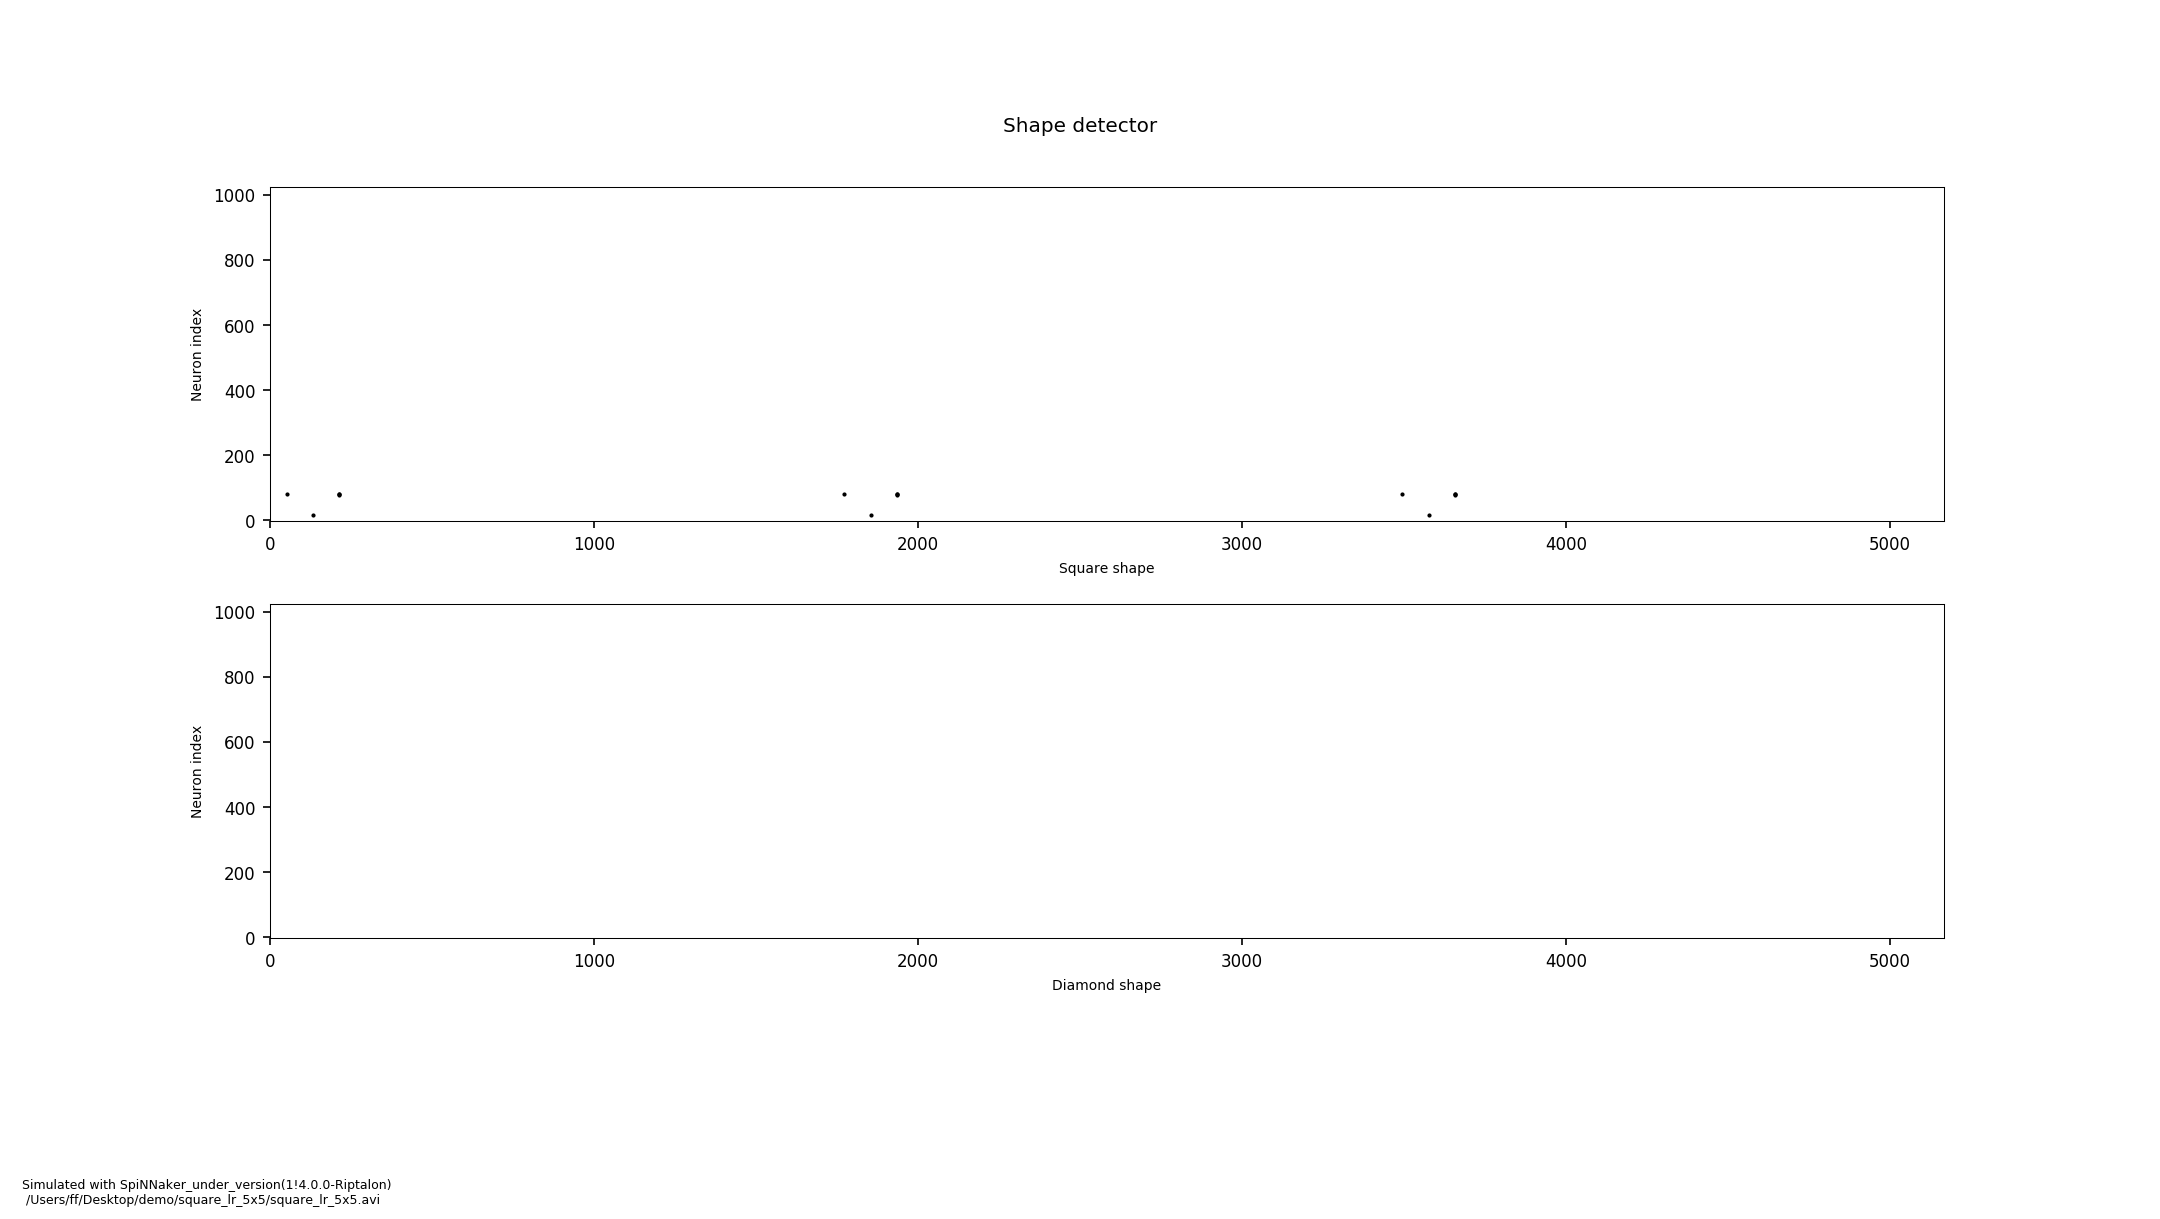
\includegraphics[width=0.75\textwidth]{images/appendix_evaluation/square_lr_shape.png}
\caption{Shapes detector.}
\label{fig:square_lr_shape}
\end{subfigure}

\caption[$5\times 5$ Square Moving Left to Right]{Screenshot and spike trains for the cells populations for a $5\times 5$ square moving from left to right. The video has been generated using a Python script.}
\label{fig:square_lr_ev}
\end{figure}


%%%%%%%%%%%%%%
\begin{figure}[ht]
\centering

\begin{subfigure}{\textwidth}
\centering
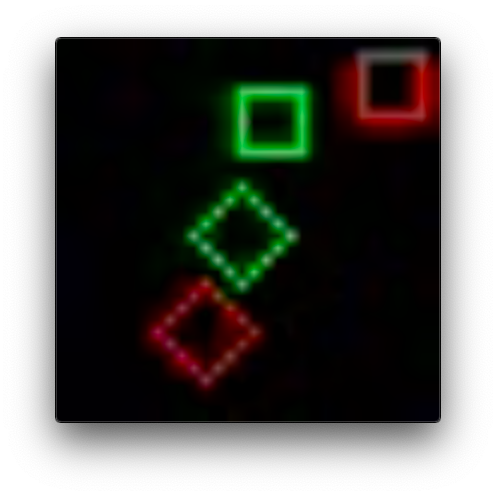
\includegraphics[width=0.3\textwidth]{images/appendix_evaluation/random_spikes.png}
\caption{DVS emulator spikes superimposed over a frame of the video.}
\label{fig:random_spikes}
\end{subfigure}

\begin{subfigure}{\textwidth}
\centering
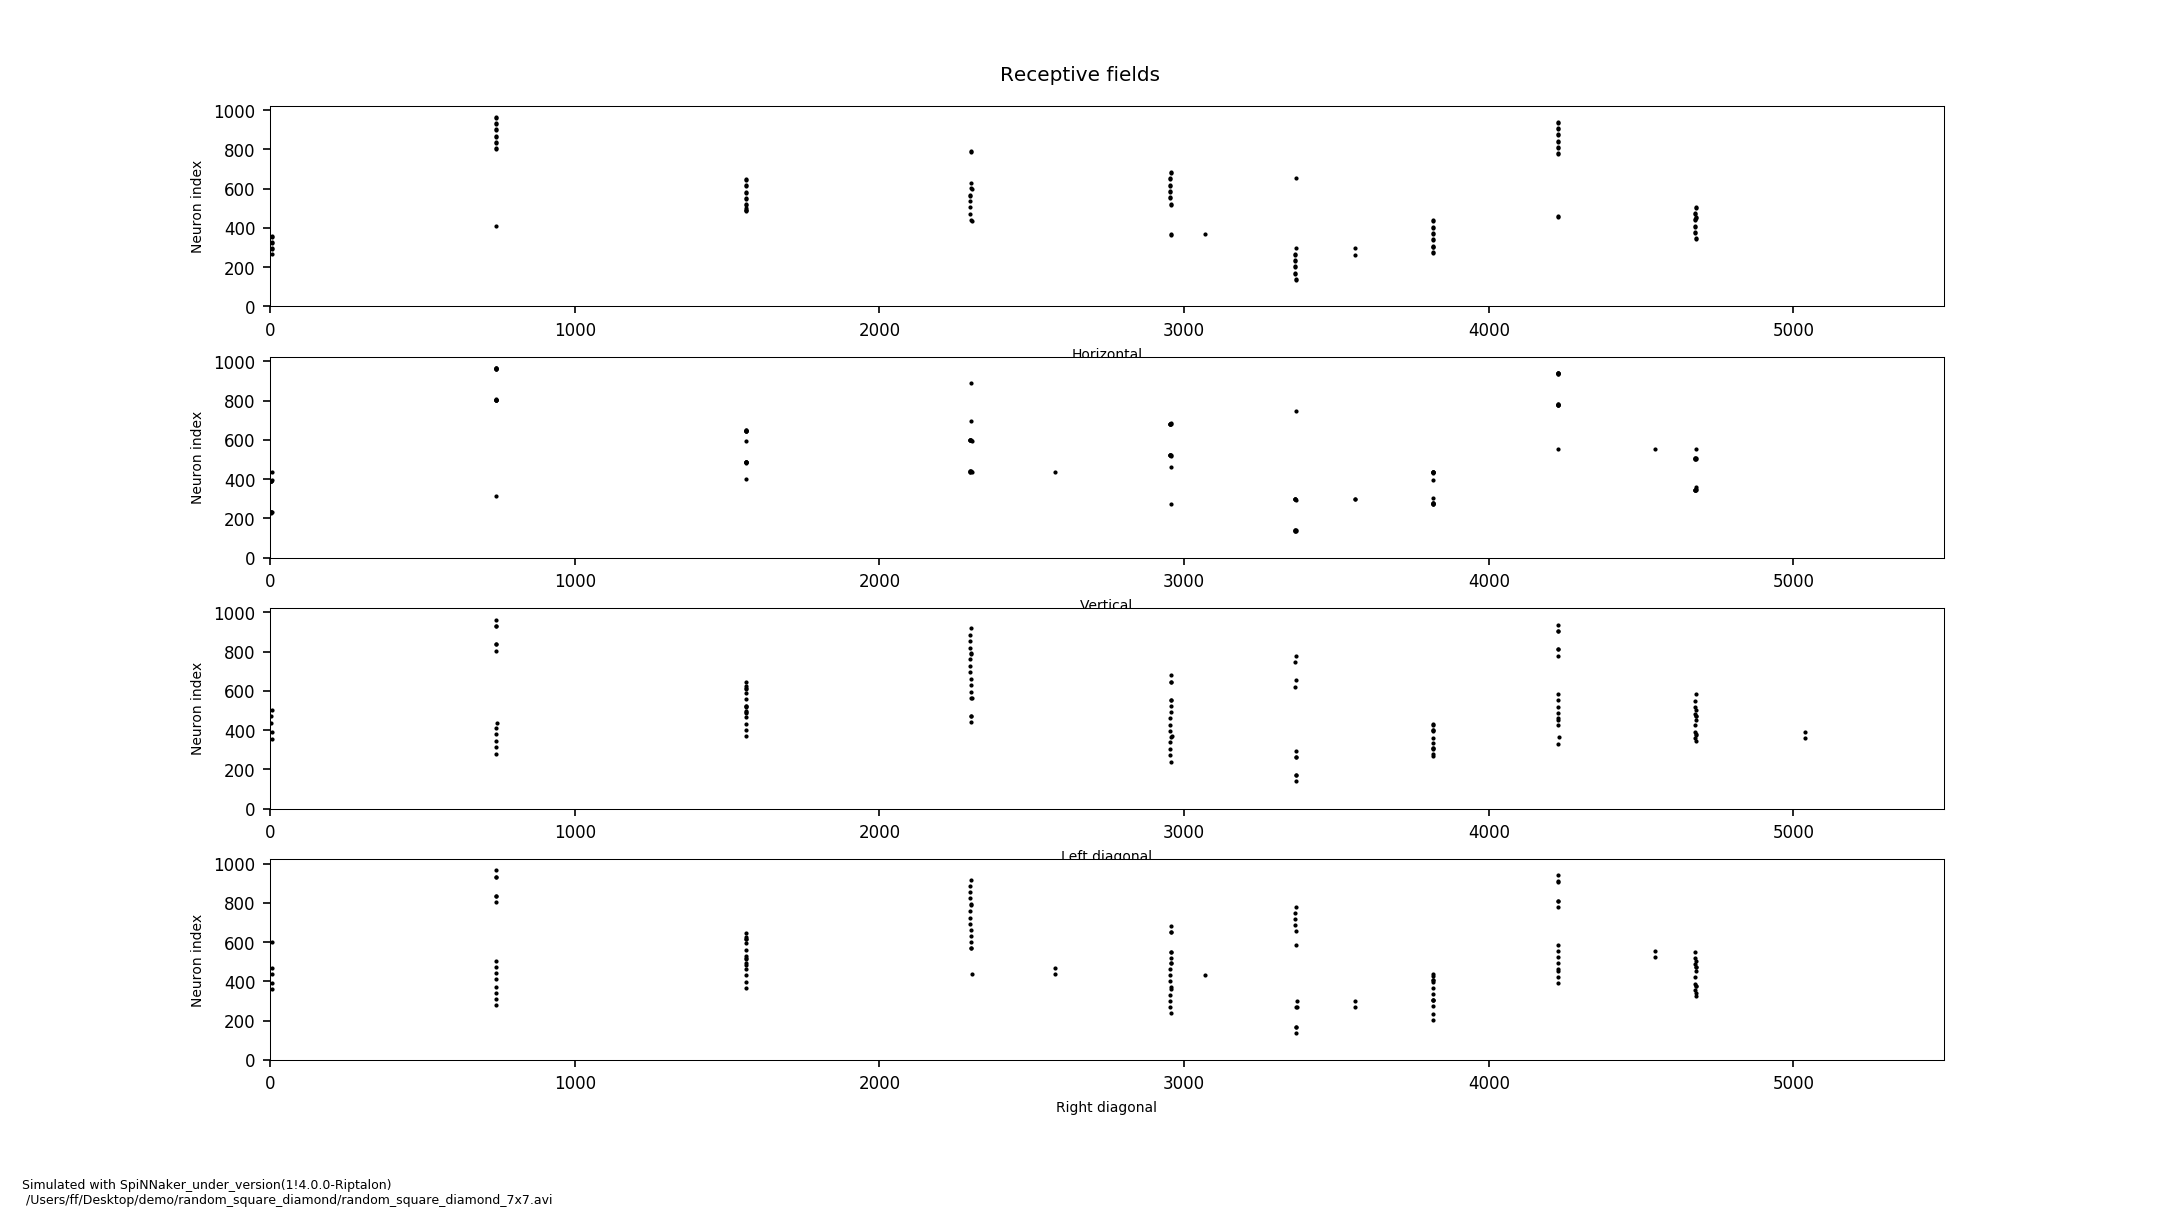
\includegraphics[width=0.75\textwidth]{images/appendix_evaluation/random_receptive_fields.png} 
\caption{Edge detectors.}
\label{fig:random_receptive_fields}
\end{subfigure}

\begin{subfigure}{\textwidth}
\centering
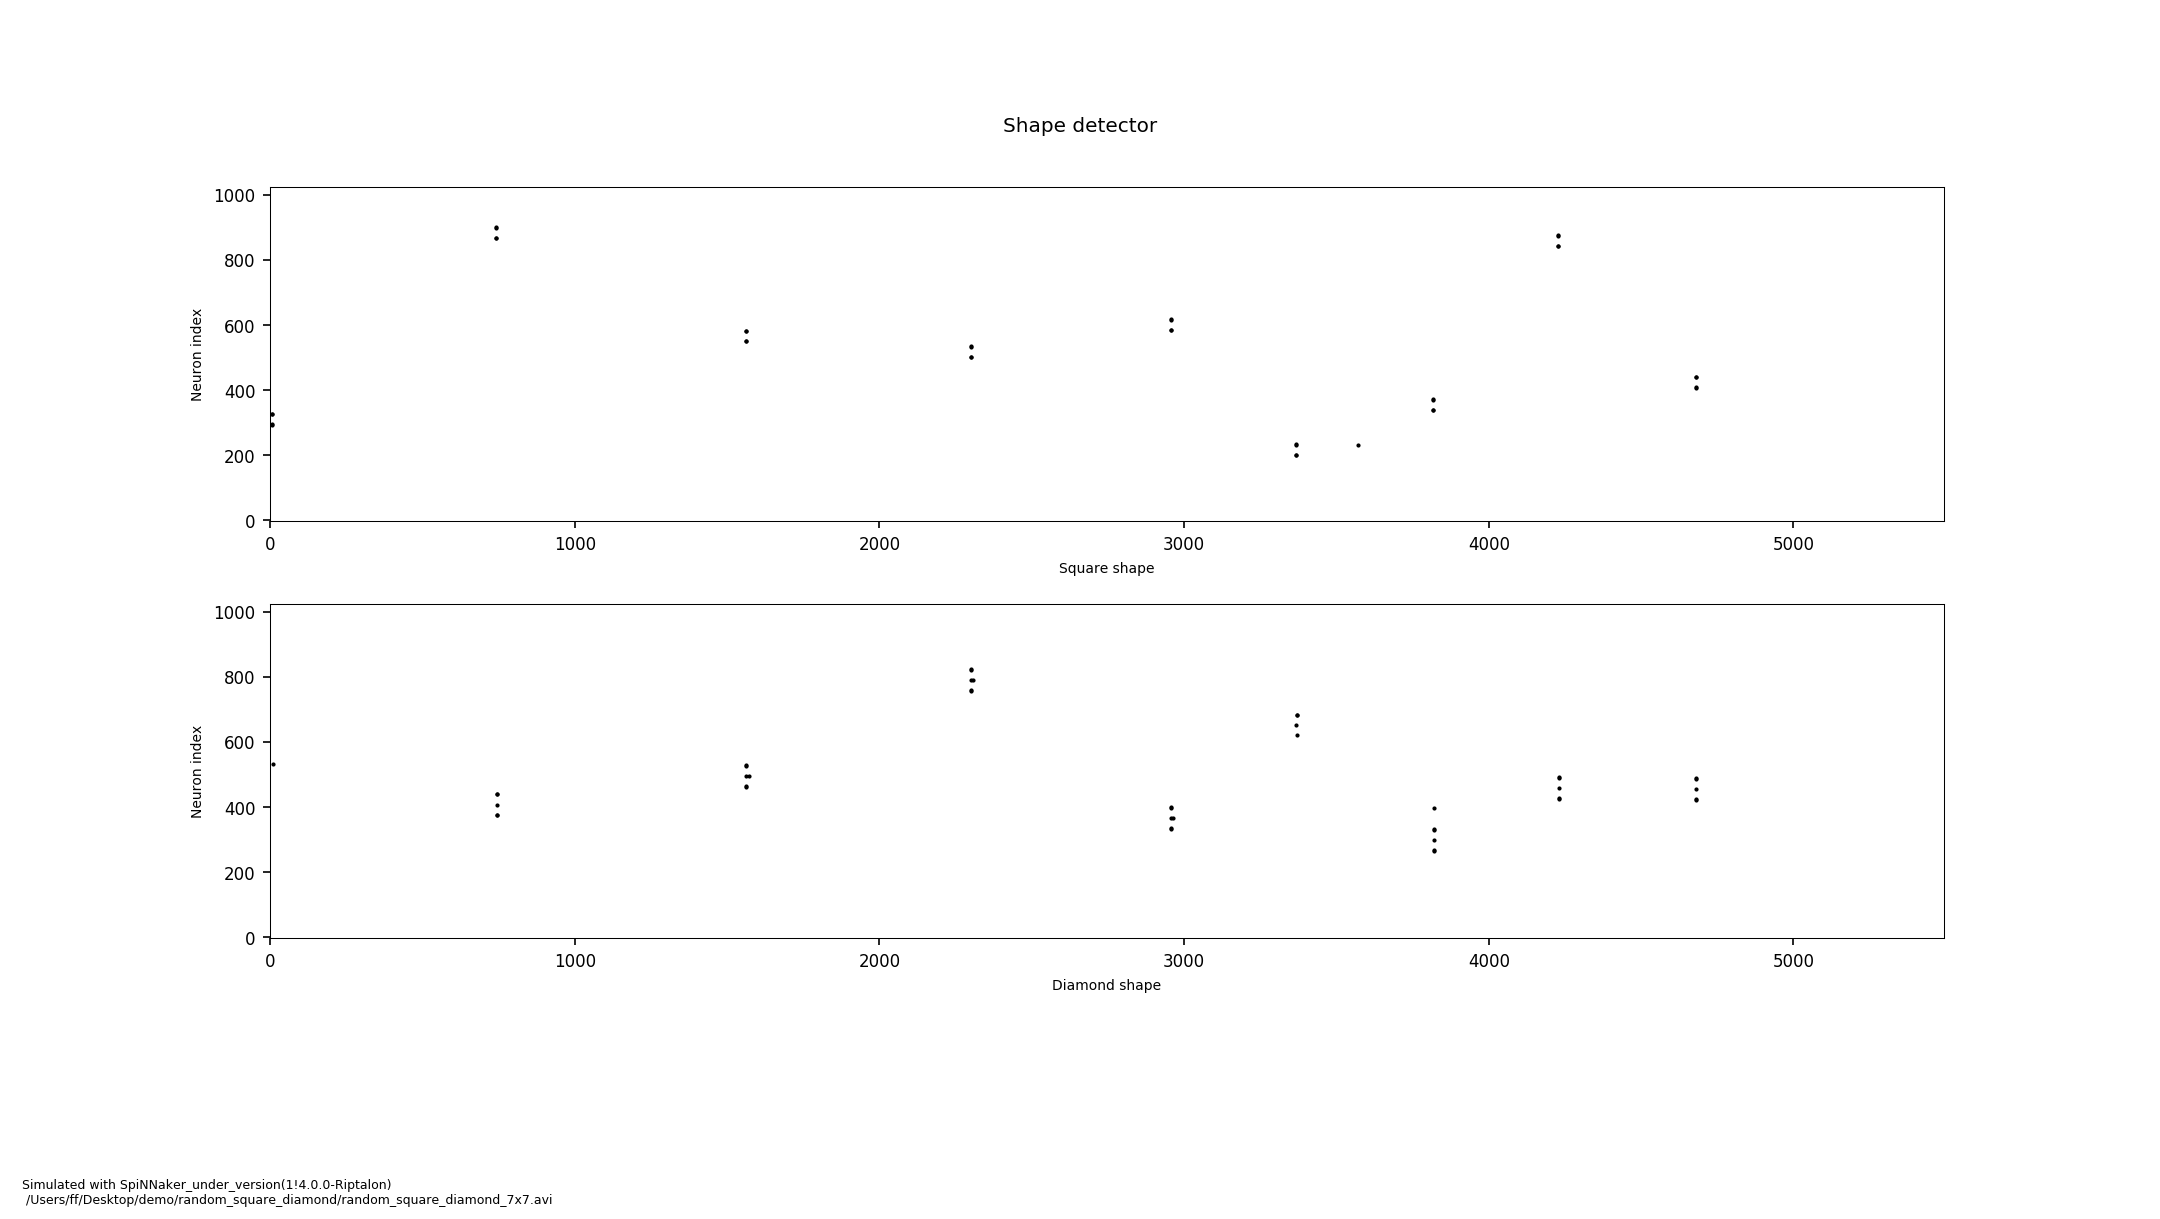
\includegraphics[width=0.75\textwidth]{images/appendix_evaluation/random_shape.png}
\caption{Shapes detector.}
\label{fig:random_shape}
\end{subfigure}

\caption[Square and Diamond Moving Randomly]{Screenshot and spike trains for the cells populations for a $5\times 5$ square and a $5\times 5$ diamond appearing at random locations. The video has been generated using a Python script.}
\label{fig:random_ev}
\end{figure}


%%%%%%%%%%%%%%%%%%%
\begin{figure}[ht]
\centering

\begin{subfigure}{\textwidth}
\centering
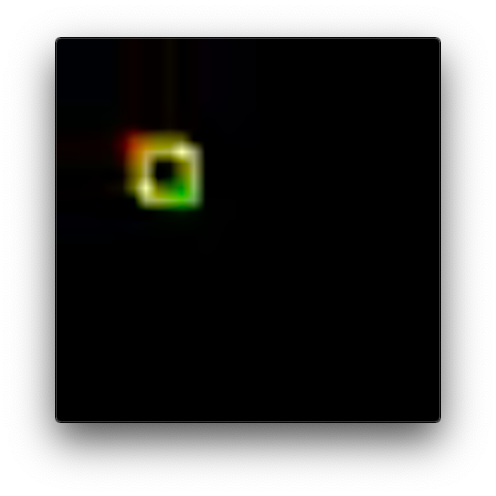
\includegraphics[width=0.3\textwidth]{images/appendix_evaluation/square_diag_spikes.png}
\caption{DVS emulator spikes superimposed over a frame of the video.}
\label{fig:square_diag_spikes}
\end{subfigure}

\begin{subfigure}{\textwidth}
\centering
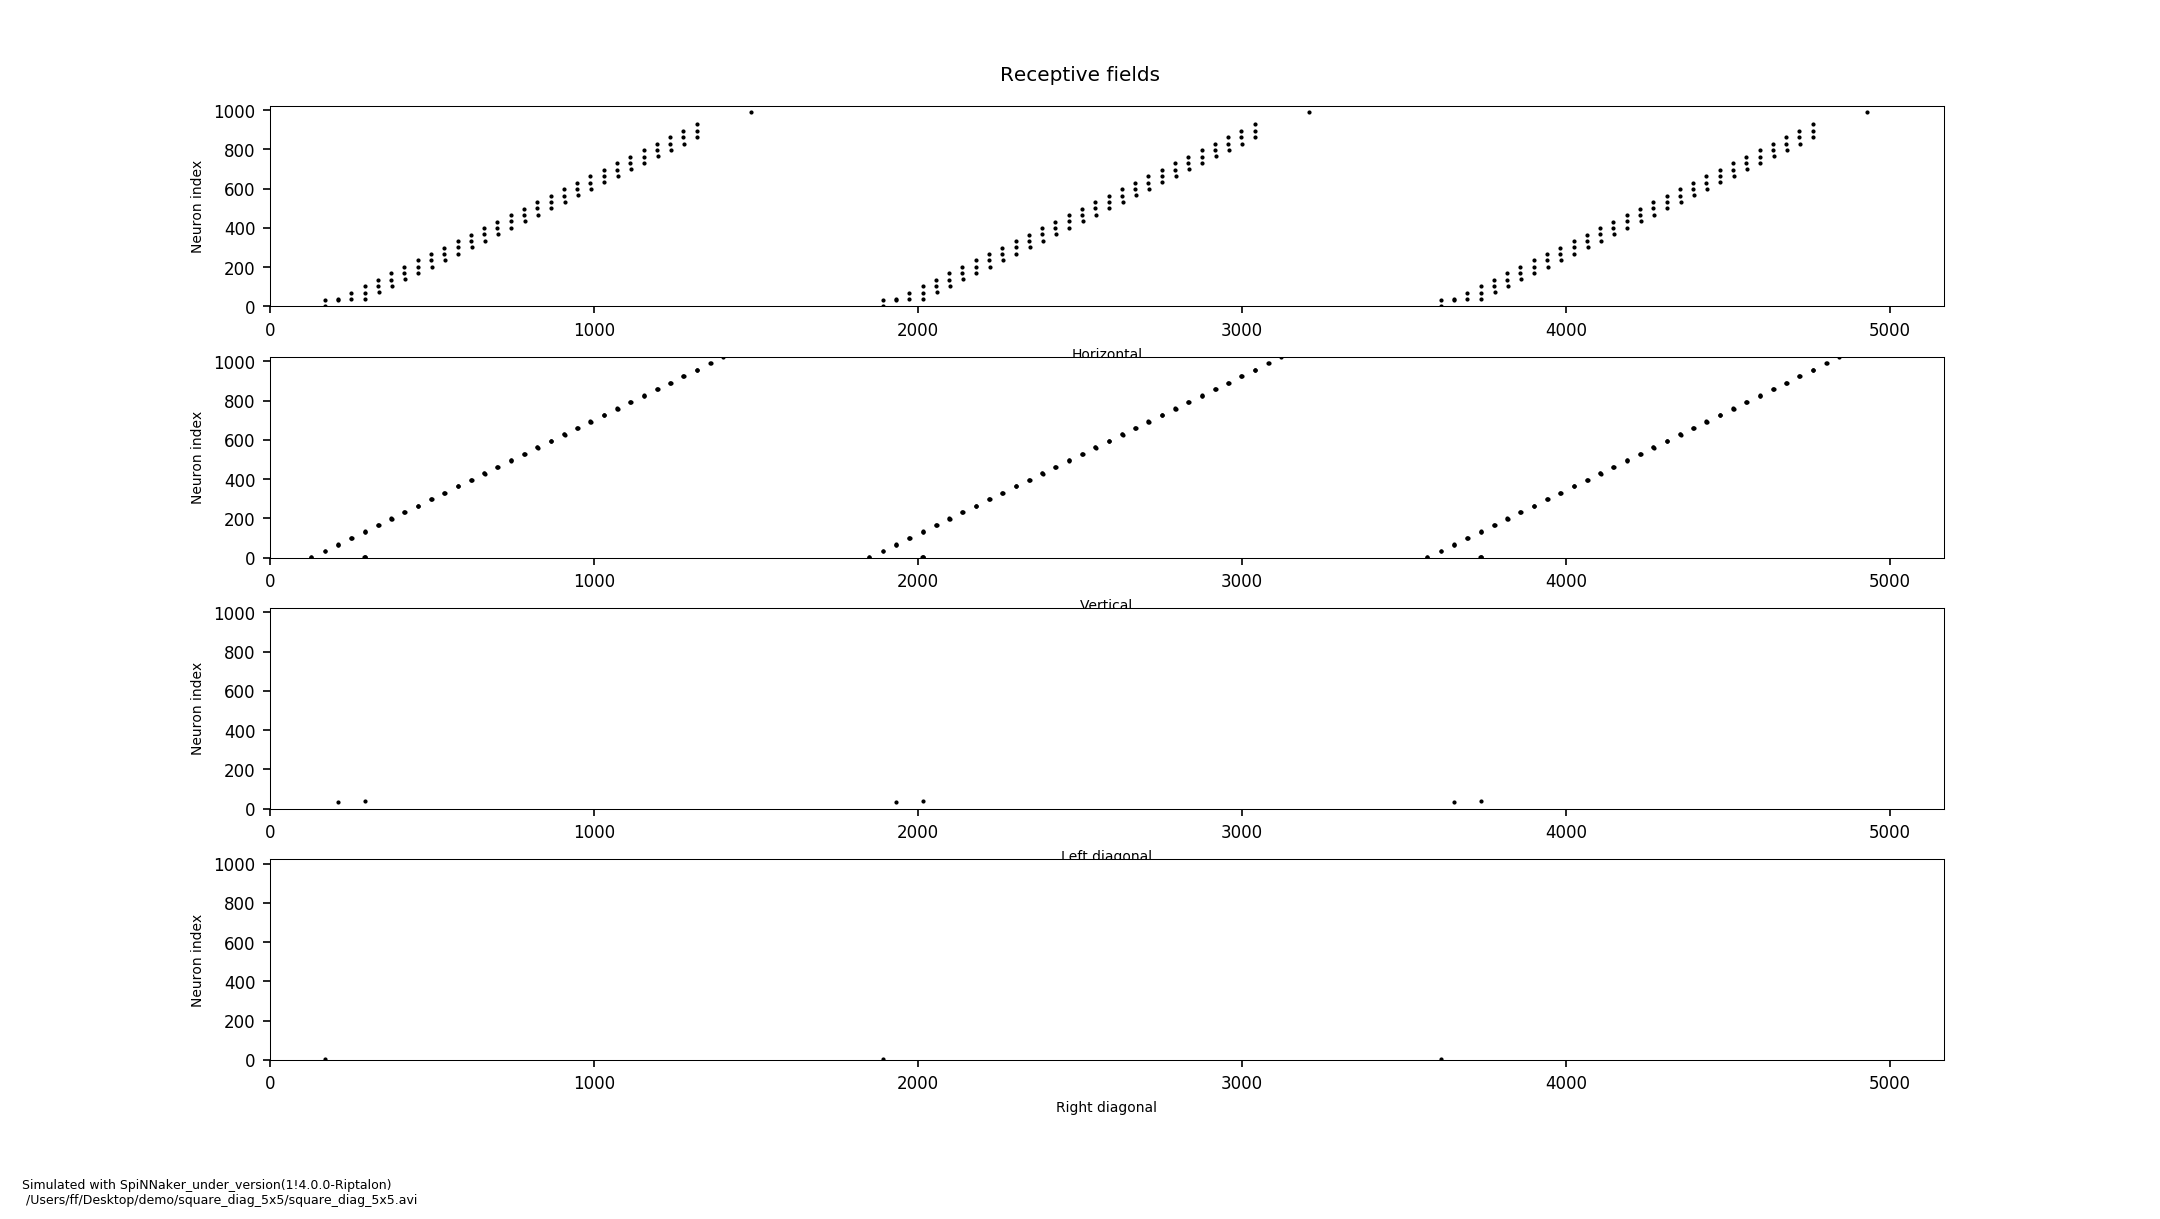
\includegraphics[width=0.75\textwidth]{images/appendix_evaluation/square_diag_receptive_fields.png} 
\caption{Edge detectors.}
\label{fig:square_diag_receptive_fields}
\end{subfigure}

\begin{subfigure}{\textwidth}
\centering
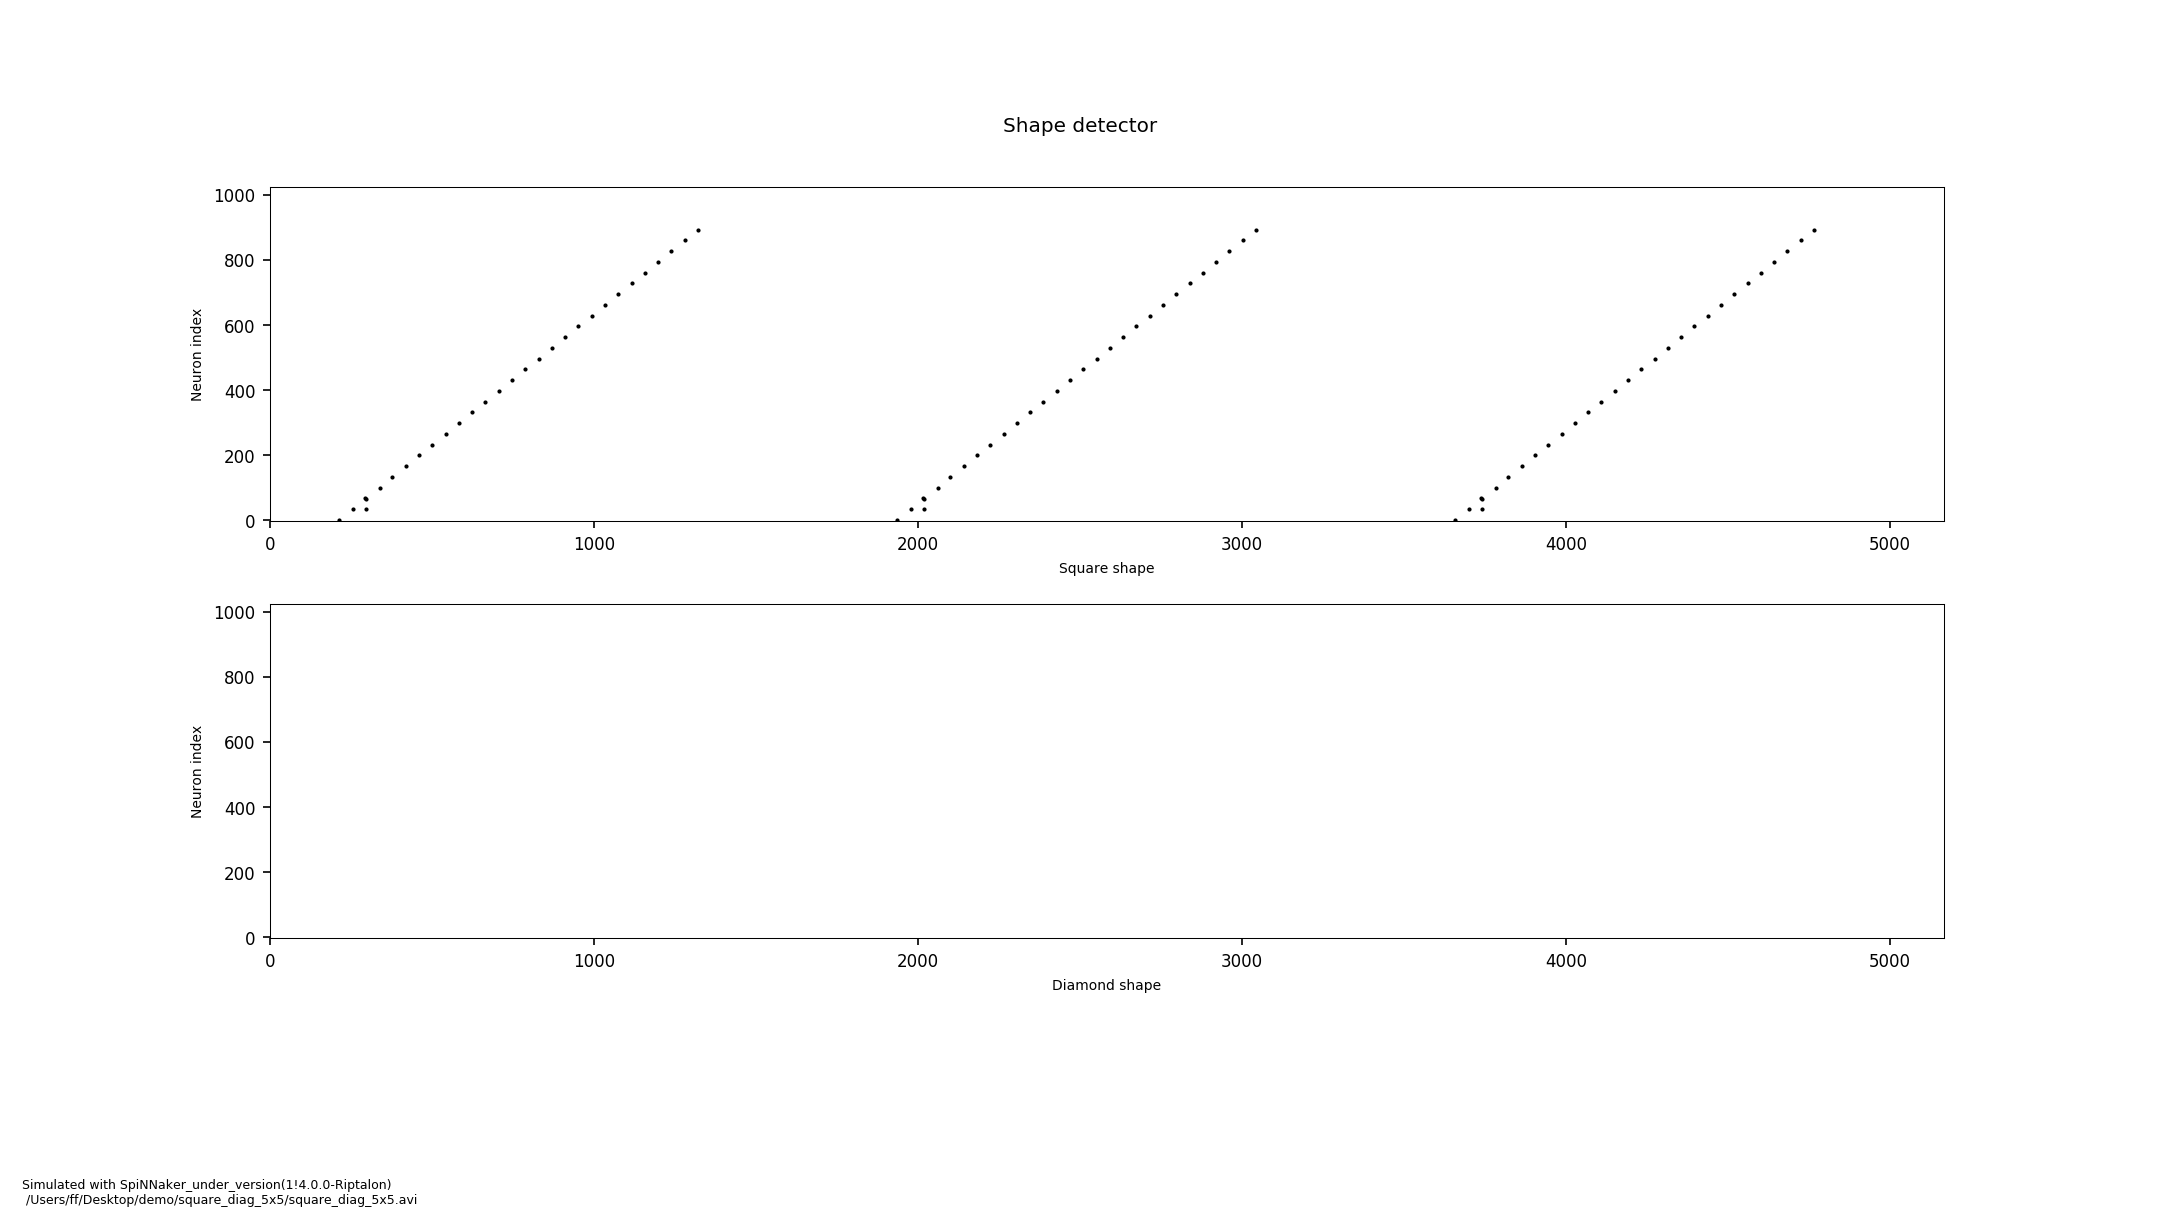
\includegraphics[width=0.75\textwidth]{images/appendix_evaluation/square_diag_shape.png}
\caption{Shapes detector.}
\label{fig:square_diag_shape}
\end{subfigure}

\caption[$5\times 5$ Square Moving Diagonally]{Screenshot and spike trains for the cells populations for a $5\times 5$ square moving from the top left corner to the bottom right corner. The video has been generated using a Python script.}
\label{fig:square_diag_ev}
\end{figure}


\end{document}
